% ============================================================================
%  Informe técnico -- Proyecto integrador Módulo 1217 (Redes Complejas)
%  Universidad de Cuenca -- Maestría en Ciencias de la Ingeniería Eléctrica
%  Compilar con:  pdflatex informe.tex  (x3, por el índice y las referencias)
% ============================================================================
\documentclass[10pt,a4paper]{extarticle}

\usepackage[utf8]{inputenc}
\usepackage[T1]{fontenc}
\usepackage{lmodern}
\usepackage[spanish,es-noindentfirst,es-tabla]{babel}
\usepackage[margin=2.3cm,top=2.3cm,bottom=2.1cm]{geometry}
\linespread{0.97}\selectfont
\usepackage{graphicx}
\usepackage{booktabs}
\usepackage{array}
\usepackage{longtable}
\usepackage{multirow}
\usepackage{makecell}
\usepackage{adjustbox}
\usepackage{xcolor}
\usepackage{amsmath}
\usepackage{amssymb}
\usepackage{enumitem}
\usepackage{float}
\usepackage{titlesec}
\usepackage{caption}
\usepackage{fancyhdr}
\usepackage{parskip}
\usepackage{microtype}
\usepackage[hidelinks]{hyperref}

\definecolor{azulucuenca}{RGB}{0,42,84}
\definecolor{rojoucuenca}{RGB}{160,26,36}
\definecolor{grisclaro}{RGB}{242,244,247}

\hypersetup{
  colorlinks=true, linkcolor=azulucuenca, citecolor=azulucuenca,
  urlcolor=rojoucuenca,
  pdftitle={Análisis de Redes Complejas -- Red de datos de la Universidad de Cuenca},
  pdfauthor={Efrain Adolfo Alvarado Plasencia}
}

\titleformat{\section}{\normalfont\Large\bfseries\color{azulucuenca}}{\thesection}{0.8em}{}
\titleformat{\subsection}{\normalfont\large\bfseries\color{azulucuenca}}{\thesubsection}{0.8em}{}
\titleformat{\subsubsection}{\normalfont\bfseries}{\thesubsubsection}{0.8em}{}

\graphicspath{{../analisis/figuras/}}
\setlength{\tabcolsep}{4pt}
\renewcommand{\arraystretch}{1.05}
\sloppy

\pagestyle{fancy}
\fancyhf{}
\renewcommand{\headrulewidth}{0.4pt}
\fancyhead[L]{\small\textcolor{rojoucuenca}{\textbf{PROYECTO: RED UCUENCA}}}
\fancyhead[R]{\small\textcolor{azulucuenca}{UNIVERSIDAD DE CUENCA}}
\fancyfoot[C]{\thepage}

\newcommand{\code}[1]{\texttt{\small #1}}
\captionsetup{font=small,labelfont={bf,color=azulucuenca}}

% Caja de "idea clave" (tcolorbox)
\usepackage[most]{tcolorbox}
\newtcolorbox{clave}{colback=grisclaro,colframe=azulucuenca,boxrule=0.7pt,
  left=3mm,right=3mm,top=2mm,bottom=2mm,arc=1mm,before skip=3mm,after skip=3mm}

% Compactar espaciado vertical
\setlength{\parskip}{2.2pt plus 1pt}
\captionsetup{skip=4pt}
\setlength{\textfloatsep}{8pt plus 2pt minus 2pt}
\setlength{\intextsep}{8pt plus 2pt minus 2pt}
\setlength{\abovedisplayskip}{5pt}
\setlength{\belowdisplayskip}{5pt}
\titlespacing*{\section}{0pt}{10pt}{5pt}
\titlespacing*{\subsection}{0pt}{8pt}{3pt}
\titlespacing*{\subsubsection}{0pt}{6pt}{2pt}

\begin{document}

% ============================================================================
% PORTADA
% ============================================================================
\begin{titlepage}
\thispagestyle{empty}
\begin{center}
\vspace*{5mm}
{\Large\textbf{\textcolor{azulucuenca}{UNIVERSIDAD DE CUENCA}}}\\[3mm]
{\large Maestría en Ciencias de la Ingeniería Eléctrica --- IV Cohorte}\\[1.5mm]
{\large Módulo 1217 --- Redes Complejas (3,5 créditos)}\\[22mm]

{\large\textsc{Proyecto integrador del módulo}}\\[8mm]

\textcolor{azulucuenca}{\rule{0.85\textwidth}{1.2pt}}\\[5mm]
{\Huge\bfseries\textcolor{azulucuenca}{Análisis de Redes Complejas}}\\[5mm]
{\Large\bfseries Caso de estudio: la red de datos\\[1mm] de la Universidad de Cuenca}\\[5mm]
\textcolor{azulucuenca}{\rule{0.85\textwidth}{1.2pt}}\\[8mm]

{\normalsize\itshape Diagnóstico de puntos críticos y propuesta de rediseño acotada\\
sobre un grafo de 177 nodos y 209 enlaces reconstruido a partir de los 34 diagramas\\
del informe técnico institucional de topologías y conexiones de red}\\[22mm]

\begin{adjustbox}{max width=\textwidth}
\begin{tabular}{ll}
\textbf{Integrante:} & Efrain Adolfo Alvarado Plasencia \\[1.5mm]
\textbf{Correo institucional:} & \href{mailto:efrain.alvarado@ucuenca.edu.ec}{efrain.alvarado@ucuenca.edu.ec} \\[1.5mm]
\textbf{Repositorio de código:} & \url{https://github.com/chino111160/redes-complejas-ucuenca} \\[1.5mm]
\textbf{Docente:} & Dr. Fabián Astudillo-Salinas \\
\end{tabular}

\vspace{25mm}
\end{adjustbox}

\vfill
{\large Cuenca --- Ecuador}\\[2mm]
{\large Agosto de 2026}
\end{center}
\end{titlepage}

% ============================================================================
\pagenumbering{roman}
\tableofcontents
\newpage
\pagenumbering{arabic}
\setcounter{page}{1}

% ============================================================================
\section*{Resumen ejecutivo}
\addcontentsline{toc}{section}{Resumen ejecutivo}
\markboth{}{}

\textbf{Problema.} La red de datos de la Universidad de Cuenca ---177 equipos y 209
enlaces distribuidos en seis campus y dos sedes, interconectados por una nube MPLS de
proveedor--- se modela como un grafo simple, no dirigido y conexo para responder una
pregunta de ingeniería concreta: \textit{¿cuáles son los puntos críticos de la red, qué
tan grave sería su falla, y qué intervenciones acotadas mejorarían más su robustez y su
desempeño?}

\textbf{Método.} Se recorrieron las cinco fases del módulo sobre el grafo real:
caracterización estructural y contraste con modelos nulos (Fase 1); recorridos BFS/DFS y
partición en comunidades con Louvain y $k$-means espectral (Fase 2); caminos más cortos
con Dijkstra y Floyd-Warshall, flujo máximo con Ford-Fulkerson y Edmonds-Karp, flujo de
costo mínimo y localización de instalaciones $p$-mediana / $p$-centro (Fase 3);
percolación de nodos y enlaces, cascadas de sobrecarga de Motter-Lai, epidemias SIR y un
índice compuesto de criticidad (Fase 4); y una propuesta de rediseño de cinco
intervenciones cuantificada y comparada contra alternativas ingenuas (Fase 5). Todos los
algoritmos centrales se implementaron desde cero en Julia; las bibliotecas se usaron
únicamente para verificación cruzada.

\textbf{Cuatro hallazgos principales.}

\begin{enumerate}[leftmargin=*,itemsep=2mm]
\item \textbf{El informe técnico institucional sobreestima la redundancia de Campus
Paraíso.} Sus seis nodos de agregación cuelgan de un \textit{único} core (\code{CPAR-C10})
por enlaces simples: es agregación de puertos, no redundancia de núcleo. La consecuencia
es medible: pese a tener 35 equipos de acceso (el segundo campus más grande), su flujo
máximo hacia Internet es de apenas \textbf{1\,000 Mbps}, contra 44\,000 de Central y
23\,000 de Balzay. Su corte mínimo es una sola arista.

\item \textbf{La red es robusta ante fallos aleatorios y extremadamente frágil ante
ataques dirigidos.} El umbral de percolación cae de $f_c \approx 0{,}243$ (fallo
aleatorio) a $f_c \approx 0{,}023$ (ataque por grado o por intermediación recalculada):
eliminar deliberadamente 4 de 177 equipos hace lo que al azar exige eliminar 43. La
eficiencia global se degrada aún antes: con solo el 5\,\% de los nodos atacados cae al
14,3\,\% de su valor original.

\item \textbf{La fragilidad de esta red es de conectividad, no de sobrecarga en cadena
---aunque cuando el disparador es del núcleo, el daño en capacidad sí es severo.} Bajo el
modelo de cascada de Motter-Lai (barrido de 13 valores de $\tau$), ningún nodo individual
desencadena un colapso mayor al 8,5\,\% de los \textit{equipos} de la red, ni siquiera con
margen de tolerancia $\tau = 0$. Pero medido en \textit{capacidad} (Mbps) en vez de en
número de equipos, nueve de los quince nodos candidatos superan el 20\,\% de la red incluso
con márgenes generosos ---porque los candidatos son, por construcción, los nodos \textit{core}
y WAN que concentran los enlaces troncales de mayor capacidad.

\item \textbf{47 puntos de articulación y 141 puentes} ---el 67,5\,\% de los enlaces---
sostienen una red con \textit{clustering} casi nulo (0,0952) y asortatividad negativa
($-0{,}1468$): una jerarquía \textit{core}-agregación-acceso con muy poca redundancia
estructural fuera del núcleo.
\end{enumerate}

\textbf{Recomendación.} Con cinco intervenciones acotadas ---duplicar a 10 Gbps el enlace
de salida de Paraíso, dar una segunda ruta a Hospitalidad, al Consultorio Jurídico y a
Yanuncay, y mitigar el punto más cargado de Balzay--- el flujo máximo de Paraíso se
multiplica por diez, los puentes bajan un 2,1\,\%, la distancia media un 3,1\,\% y la
eficiencia global sube un 3,5\,\%. La propuesta supera con claridad a dos alternativas
ingenuas de referencia (unir los nodos de mayor grado, o cinco enlaces al azar), que
mejoran métricas promedio sin reparar ningún cuello de botella real. \textbf{Si se
tuviera presupuesto para cinco enlaces, habría que empezar por Campus Paraíso.}

\newpage

% ============================================================================
\section{Introducción}

\subsection{El caso de estudio}

El informe técnico institucional \textit{«Diagramas de red final»} documenta, mediante 34
diagramas (\textit{weathermaps} de monitoreo más el diagrama de interconexión MPLS), la
topología de los seis campus de la Universidad de Cuenca ---Central, Balzay, Yanuncay,
Hospitalidad y Paraíso, más las sedes Museo y Centro Histórico--- y de la nube MPLS que
los interconecta. A partir de esos diagramas se reconstruyó un grafo \textbf{simple, no
dirigido y conexo} de 177 nodos y 209 aristas, saneado de 61 inconsistencias heredadas de
la transcripción original (identificadores duplicados, aristas repetidas y un atributo que
mezclaba tráfico con capacidad).

Cada nodo lleva tres atributos relevantes para el análisis: \code{campus} (ubicación
física), \code{capa} (posición en la jerarquía declarada por el informe: \code{core},
\code{agregacion}, \code{acceso}, \code{wan} o \code{interconexion}) y \code{diagrams}
(diagrama de procedencia). Cada arista lleva \code{trafico\_mbps} (medición instantánea
del monitor, definida en 170 de 209 aristas), \code{capacidad\_mbps} (capacidad nominal,
declarada explícitamente solo en las 28 aristas del diagrama MPLS) y \code{rol}
(\code{principal}, \code{wan}, \code{respaldo}, \code{secundario} o \code{inferido}).

\begin{table}[H]
\centering
\caption{Composición del grafo por capa jerárquica y por ubicación}
\label{tab:composicion}
\small
\begin{adjustbox}{max width=\textwidth}
\begin{tabular}{lr@{\hspace{18mm}}lr}
\toprule
\textbf{Capa} & \textbf{Nodos} & \textbf{Ubicación} & \textbf{Nodos} \\
\midrule
\code{acceso}       & 132 & Campus Central        & 75 \\
\code{agregacion}   &  27 & Campus Paraíso        & 44 \\
\code{wan}          &  11 & Campus Balzay         & 35 \\
\code{core}         &   5 & Campus Yanuncay       & 13 \\
\code{interconexion}&   2 & Campus Hospitalidad   &  5 \\
                    &     & Sede Museo            &  2 \\
                    &     & Sede Centro Histórico &  2 \\
                    &     & Nube MPLS             &  1 \\
\midrule
\textbf{Total} & \textbf{177} & \textbf{Total} & \textbf{177} \\
\bottomrule
\end{tabular}
\end{adjustbox}
\end{table}

De las 209 aristas, 157 tienen \code{rol=principal}, 32 \code{rol=wan}, 12
\code{rol=respaldo}, 5 \code{rol=secundario} y 3 \code{rol=inferido}. Solo
\textbf{17 aristas cruzan la frontera entre dos campus}: la institución es, topológicamente,
un conjunto de siete islas cosidas por un puñado de enlaces WAN. Esa observación
elemental anticipa buena parte de los resultados de las secciones siguientes.

\subsection{Las preguntas que responde este informe}

El enunciado del proyecto plantea una pregunta general que amarra las cinco fases:
\textit{¿cuáles son los puntos críticos de la red de datos de la Universidad de Cuenca,
qué tan grave sería su falla, y qué intervenciones concretas ---acotadas en número y
justificadas con métricas--- mejorarían más su robustez y su desempeño?} Cada sección de
este informe resuelve un subconjunto de los once problemas (P1--P11) y aporta una pieza de
esa respuesta; la Sección~\ref{sec:conclusiones} las integra.

Además, el proyecto exige contrastar los datos con lo que \textit{afirma} el informe
técnico institucional. Ese contraste produjo el hallazgo más accionable del trabajo
(Sección~\ref{sec:contraste}) y es la base directa de la primera intervención propuesta.

\subsection{Metodología y decisiones de modelado}

El análisis se organiza en cinco fases encadenadas, cada una apoyada en los resultados de
la anterior. Las decisiones de modelado que condicionan los resultados son cuatro y se
declaran aquí de forma explícita para que el lector pueda juzgarlas:

\begin{enumerate}[leftmargin=*,itemsep=1.5mm]
\item \textbf{Grafo simple no dirigido.} Un enlace físico entre dos equipos se modela como
una arista, sin dirección y sin multiplicidad. La consecuencia práctica ---discutida en la
Sección~\ref{sec:p11}--- es que \textit{duplicar} una fibra entre el mismo par de equipos
no crea una arista nueva: aumenta capacidad, no redundancia topológica.

\item \textbf{Tres modelos de peso alternativos} (P5): $w_{\text{saltos}} = 1$,
$w_{\text{latencia}} = \alpha + \beta/c(u,v)$ y $w_{\text{carga}} = b(u,v)/c(u,v)$. No se
elige uno «correcto»: se calculan los tres y se compara qué cambia, porque cada uno
responde a una pregunta distinta.

\item \textbf{Estimación de capacidad documentada arista por arista} (P6.1). La capacidad
nominal solo consta en 28 de 209 aristas; las 181 restantes se estiman con reglas
explícitas y se registra el supuesto usado en cada una. Toda conclusión sobre flujo
depende de esas reglas, y así se señala.

\item \textbf{Implementación propia de los algoritmos centrales.} BFS, DFS, Dijkstra
(con montículo binario propio), Floyd-Warshall, Louvain, $k$-means, Tarjan (puentes y
articulación), modelo de configuración, NMI/ARI, percolación, cascadas y SIR se
programaron desde cero. \code{Graphs.jl} se usa solo para verificación cruzada, y
Ford-Fulkerson / Edmonds-Karp / $k$-means se reutilizan del código de referencia del
módulo, citando la procedencia.
\end{enumerate}

\subsection{Reproducibilidad}

Todos los números de este informe se generan ejecutando, en orden, los cinco
\textit{scripts} de \code{analisis/scripts/} sobre el entorno Julia declarado en
\code{analisis/Project.toml}. Cada \textit{script} verifica automáticamente la carga de
datos contra los trece valores de referencia del Anexo A del enunciado \textit{antes} de
calcular nada, y aborta si alguno no coincide. Las tablas y figuras completas quedan en
\code{analisis/resultados/} y \code{analisis/figuras/}. El detalle de ejecución está en el
Anexo~\ref{anx:repro}.

% ============================================================================
\section{Caracterización estructural (Fase 1)}

\textit{Unidad 1 del sílabo. Problemas P1 (medidas fundamentales) y P2 (modelos nulos y
visualización).}

\subsection{P1 --- Medidas fundamentales}

\subsubsection{Medidas globales}

\begin{table}[H]
\centering
\caption{Medidas globales de la red UCuenca}
\label{tab:globales}
\small
\begin{adjustbox}{max width=\textwidth}
\begin{tabular}{lr}
\toprule
\textbf{Métrica} & \textbf{Valor} \\
\midrule
Nodos ($n$)                       & 177 \\
Aristas ($m$)                     & 209 \\
Densidad $2m/[n(n-1)]$            & 0,0134 \\
Componentes conexas               & 1 (tamaño 177) \\
Grado medio / máximo / mínimo     & 2,36 / 17 / 1 \\
Coeficiente de \textit{clustering} medio & 0,0952 \\
Diámetro                          & 11 \\
Distancia media entre pares       & 5,830 \\
Asortatividad por grado           & $-0{,}1468$ \\
Puntos de articulación            & 47 \\
Puentes                           & 141 (67,5\,\% de las aristas) \\
Número ciclomático $m-n+c$        & 33 \\
\bottomrule
\end{tabular}
\end{adjustbox}
\end{table}

Con densidad 0,0134 la red es extremadamente dispersa: de los $\binom{177}{2} = 15\,576$
pares posibles solo 209 están conectados. Un nodo típico tiene dos o tres vecinos. Esto es
exactamente lo esperable de una red de infraestructura física jerárquica ---no de una red
social ni de una red aleatoria densa--- y explica de raíz el resto de las medidas.

\textbf{¿Por qué el \textit{clustering} es tan bajo comparado con el de una red social?}
El coeficiente de \textit{clustering} mide la probabilidad de que dos vecinos de un nodo
sean vecinos entre sí ---el «cierre triádico». En una red social esa probabilidad es alta
(típicamente $C \sim 0{,}3$--$0{,}6$) porque los amigos de una persona tienden a conocerse:
el mecanismo generador es social y favorece los triángulos. En una jerarquía
\textit{core}-agregación-acceso el mecanismo generador es el opuesto: un equipo de acceso
se conecta a \textit{su} switch de agregación y, con suerte, a un enlace de respaldo; dos
equipos de acceso colgados del mismo switch \textit{no} se conectan entre sí, porque
hacerlo no aporta nada al diseño y sí consume puertos. El valor medido, 0,0952, no es un
defecto de la red: es la firma de una topología en estrella de estrellas. Los pocos
triángulos que existen provienen de los pares redundantes deliberados del núcleo, y la
Sección~\ref{sec:p2} demuestra cuantitativamente que son deliberados.

\textbf{¿Por qué la asortatividad es negativa y qué dice sobre la jerarquía?} La
asortatividad por grado es el coeficiente de correlación de Pearson entre los grados de
los dos extremos de cada arista (Newman, 2010, ec.~8.28). Un valor negativo
($-0{,}1468$) significa que los nodos de alto grado tienden a conectarse con nodos de bajo
grado, no entre sí: el patrón \textit{disortativo}. Y es precisamente lo que dicta la
jerarquía: un switch de agregación con 12 puertos ocupados los usa para colgar 12 equipos
de acceso de grado 1, no para conectarse a otros 12 switches de agregación. En una red
social el signo sería el contrario (los individuos muy conectados tienden a conocerse
entre ellos). El signo de esta única cifra distingue, sin ambigüedad, una red de
infraestructura diseñada de una red de crecimiento social.

\subsubsection{Distribución de grado}

\begin{figure}[tbp]
\centering
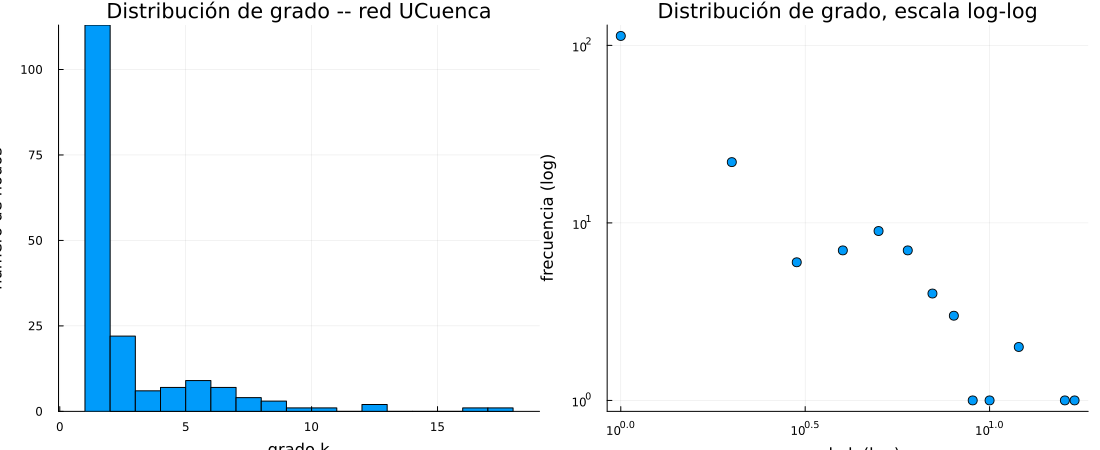
\includegraphics[width=0.58\textwidth]{p1_distribucion_grado.png}
\caption{Distribución de grado de la red UCuenca: histograma (izquierda, eje $x$ = grado
$k$, eje $y$ = número de nodos) y misma distribución en escala log-log (derecha,
frecuencia frente a grado). La cola pesada es visible pero corta: solo 4 nodos superan
grado 10.}
\label{fig:grado}
\end{figure}

\begin{table}[H]
\centering
\caption{Distribución de grado completa}
\label{tab:distgrado}
\small
\begin{adjustbox}{max width=\textwidth}
\begin{tabular}{lrrrrrrrrrrrrr}
\toprule
Grado $k$ & 1 & 2 & 3 & 4 & 5 & 6 & 7 & 8 & 9 & 10 & 12 & 16 & 17 \\
Nodos     & 113 & 22 & 6 & 7 & 9 & 7 & 4 & 3 & 1 & 1 & 2 & 1 & 1 \\
\bottomrule
\end{tabular}
\end{adjustbox}
\end{table}

Los 113 nodos de grado 1 son, casi sin excepción, equipos de acceso terminales: hojas del
árbol. En el otro extremo, \code{DATCC-2A-C3} (grado 17) y \code{DATCC-2A-C2} (grado 16)
son los dos \textit{switches} de core redundantes de Campus Central. El grado máximo es
más de siete veces el grado medio.

\textbf{¿Se observa una cola pesada? ¿Tiene sentido hablar de «red libre de escala»?} Un
ajuste exploratorio de ley de potencias por máxima verosimilitud sobre la cola
($k \ge k_{\min} = 2$, el percentil 75 de la distribución) da un exponente
$\alpha \approx 2{,}04$, un valor que en la literatura se leería como «libre de escala».
\textbf{Esa lectura sería incorrecta aquí, y conviene decir por qué.} Con $n = 177$ nodos
la muestra de la cola tiene apenas 64 observaciones, muy por debajo de lo que exige una
afirmación de ese tipo. Antes de afirmarlo haría falta el procedimiento completo de
Clauset, Shalizi y Newman (2009): (i) estimar $k_{\min}$ minimizando la distancia
Kolmogorov-Smirnov en lugar de fijarlo a un percentil arbitrario; (ii) una prueba formal de
bondad de ajuste por KS con $p$-valor obtenido por remuestreo sintético; y (iii) una
comparación por razón de verosimilitud contra alternativas plausibles ---log-normal,
exponencial, exponencial estirada---, que en muestras pequeñas suelen ajustar igual de
bien o mejor. Ninguna de las tres se ejecuta aquí porque el tamaño de muestra no lo
justifica, y el exponente se reporta únicamente como insumo descriptivo. Lo que sí es
indiscutible en los datos es la \textbf{heterogeneidad de grado}, y esa heterogeneidad
basta para explicar buena parte de lo que se ve en las secciones siguientes.

\subsubsection{Centralidades}

\begin{table}[H]
\centering
\caption{Top-10 por las cuatro centralidades (tabla comparativa única, P1.3)}
\label{tab:centralidades}
\scriptsize
\setlength{\tabcolsep}{2.6pt}
\begin{adjustbox}{max width=\textwidth}
\begin{tabular}{r|lr|lr|lr|lr}
\toprule
\# & \textbf{Grado} & Val. & \textbf{Cercanía} & Val. & \textbf{Intermediación} & Val. & \textbf{Vector propio} & Val. \\
\midrule
1  & DATCC-2A-C3          & 17 & INTERNET-MPLS            & 0,2759 & DATCC-2A-C3                & 0,4468 & DATCC-2A-C3            & 0,5022 \\
2  & DATCC-2A-C2          & 16 & DATCC-2A-C3              & 0,2683 & CPAR-C10                   & 0,4043 & DATCC-2A-C2            & 0,4818 \\
3  & AGRPRI-1A-D10        & 12 & PE2-CENTRAL              & 0,2667 & ROUTER-CAMPUS-HUAYNA-CAPAC & 0,3663 & FORTIGATE-1800F-CENTRAL& 0,2005 \\
4  & BAL-AUL2-D1          & 12 & FORTIGATE-1800F-CENTRAL  & 0,2596 & INTERNET-MPLS              & 0,3657 & CC-ARQUITECTURA-D107   & 0,1977 \\
5  & CC-ARQUITECTURA-D107 & 10 & PE1-CENTRAL              & 0,2562 & PE2-CENTRAL                & 0,2881 & CC-MONJAS-D126         & 0,1855 \\
6  & CP-EADMINA1-D6       &  9 & PE1-BALZAY               & 0,2511 & DT-0A-C13                  & 0,2235 & CC-ADM-D40             & 0,1799 \\
7  & CC-MONJAS-D126       &  8 & DATCC-2A-C2              & 0,2475 & FORTIGATE-1800F-CENTRAL    & 0,1863 & CC-ECONOMIA-D51        & 0,1751 \\
8  & DT-0A-C13            &  8 & ROUTER-HUAYNA-CAPAC      & 0,2421 & DATCC-2A-C2                & 0,1706 & CC-JURISPRUDENCIA-D110 & 0,1748 \\
9  & INTERNET-MPLS        &  8 & FORTIGATE-1800F-BALZAY   & 0,2408 & FORTIGATE-1800F-BALZAY     & 0,1490 & CC-FILOSOFIA-A-D108    & 0,1701 \\
10 & BAL-CENTEC-D2        &  7 & PE2-BALZAY               & 0,2385 & PE2-BALZAY                 & 0,1460 & CC-QUIMICA-D109        & 0,1701 \\
\bottomrule
\end{tabular}
\end{adjustbox}
\end{table}

\textbf{¿Coinciden los nodos más centrales por grado con los más centrales por
intermediación?} \textbf{No: solo 4 de los 10 coinciden}, y esa discrepancia es
informativa, no ruido. Las dos medidas responden preguntas distintas:

\begin{itemize}[leftmargin=*,itemsep=1mm]
\item El \textbf{grado} cuenta cuántos vecinos \textit{directos} tiene un equipo. Un
switch de agregación con muchos puertos ocupados (\code{AGRPRI-1A-D10},
\code{BAL-AUL2-D1}, ambos con grado 12) puntúa alto aunque nadie más pase por él.
\item La \textbf{intermediación} cuenta por cuántos caminos mínimos \textit{entre terceros}
pasa un nodo. Aquí puntúan los \textit{core} y los \textit{routers} de interconexión
(\code{DATCC-2A-C3}, \code{CPAR-C10}, \code{ROUTER-CAMPUS-HUAYNA-CAPAC},
\code{INTERNET-MPLS}), que están en el único camino posible entre campus.
\end{itemize}

El papel operativo de cada grupo es distinto y exige protección distinta. \code{BAL-AUL2-D1}
es crítico \textit{para sus diez equipos de acceso}: si cae, esos diez pierden servicio,
pero el resto de la institución ni se entera. \code{DATCC-2A-C3} o \code{CPAR-C10} son
críticos \textit{para todos los demás}: si caen, se parte la red. Un plan de continuidad
que priorice solo por número de usuarios afectados protegerá los primeros y descuidará los
segundos. La \textbf{cercanía} añade una tercera lectura: la encabeza \code{INTERNET-MPLS},
que no es el nodo de mayor grado ni el de mayor intermediación, pero sí el punto desde el
que se llega a todo lo demás en menos saltos ---consecuencia directa de ser el eje
inter-campus. La centralidad de \textbf{vector propio}, por último, premia estar conectado
a nodos que a su vez están bien conectados, y por eso su top-10 se llena de equipos de
Campus Central colgados de los dos \textit{core}: mide pertenencia al núcleo denso, no
criticidad.

\subsubsection{Puentes y puntos de articulación}
\label{sec:puentes}

De las 209 aristas, \textbf{141 (67,5\,\%) son puentes} ---aristas cuya eliminación
desconecta el grafo--- y \textbf{47 de los 177 nodos son puntos de articulación}. Ambos se
calcularon con el algoritmo de Tarjan (DFS con tiempos de descubrimiento y valores
\textit{low-link}), implementado a mano en $O(V+E)$.

\begin{table}[H]
\centering
\caption{Puentes y puntos de articulación por ubicación y por capa (P1.5)}
\label{tab:puentescampus}
\small
\begin{adjustbox}{max width=\textwidth}
\begin{tabular}{lr@{\hspace{6mm}}r@{\hspace{16mm}}lr@{\hspace{6mm}}r}
\toprule
\textbf{Campus} & \textbf{Puentes}$^\dagger$ & \textbf{Articul.} & \textbf{Capa} & \textbf{Puentes}$^\dagger$ & \textbf{Articul.} \\
\midrule
Campus Central      & 113 & 23 & \code{acceso}       & 149 & 17 \\
Campus Paraíso      &  84 & 14 & \code{agregacion}   & 122 & 26 \\
Campus Balzay       &  50 &  6 & \code{core}         &   7 &  1 \\
Campus Yanuncay     &  24 &  2 & \code{wan}          &   4 &  3 \\
Campus Hospitalidad &   9 &  1 & \code{interconexion}&   0 &  0 \\
Nube MPLS           &   2 &  1 & & & \\
\bottomrule
\multicolumn{6}{l}{\footnotesize $^\dagger$ Contando el campus/capa de cada uno de los dos extremos: la suma es $2\times 141 = 282$.}
\end{tabular}
\end{adjustbox}
\end{table}

En términos absolutos Central y Paraíso concentran los puentes simplemente porque son los
campus con más equipos. En términos \textit{relativos} la fracción de aristas que son
puentes es muy alta en todos los campus, consistente con el patrón de «árbol con pocas
redundancias» que ya anticipaban el \textit{clustering} y la asortatividad. La lectura por
capa es la que más importa operativamente: los 26 puntos de articulación de la capa de
\textbf{agregación} son el verdadero problema estructural, porque cada uno de ellos es el
único paso hacia un grupo entero de equipos de acceso. Solo hay 1 punto de articulación en
la capa \textit{core} ---el núcleo sí está bien construido---, pero eso no salva a la red:
la fragilidad se desplazó un nivel hacia abajo.

\subsubsection{Contraste con el informe técnico}
\label{sec:contraste}

El informe técnico institucional (cap.~2.1) afirma que \textbf{Balzay y Paraíso}
implementan «redundancia física completa» en los enlaces de 10 Gbps entre \textit{core} y
agregación, mientras que \textbf{Campus Central} dispone de enlaces simples entre esas
capas. Para verificarlo se contó, para cada nodo de agregación, cuántas aristas tiene
hacia nodos de capa \code{core}: dos o más significa redundancia real de núcleo; exactamente
una, enlace simple.

\begin{table}[H]
\centering
\caption{Redundancia \textit{core}-agregación observada en los datos (P1.6)}
\label{tab:redundancia}
\small
\begin{adjustbox}{max width=\textwidth}
\begin{tabular}{lrrr}
\toprule
\textbf{Campus} & \textbf{Con redundancia ($\ge 2$ enlaces)} & \textbf{Enlace simple} & \textbf{Total} \\
\midrule
Campus Balzay       &  4 & 0 &  5 \\
Campus Central      & 13 & 0 & 14 \\
\textbf{Campus Paraíso} & \textbf{0} & \textbf{6} & \textbf{6} \\
Campus Yanuncay     &  0 & 0 &  1 \\
Campus Hospitalidad &  0 & 0 &  1 \\
\bottomrule
\end{tabular}
\end{adjustbox}
\end{table}

Los datos \textbf{confirman} la redundancia de Balzay (sus cinco nodos de agregación con
datos concluyentes tienen doble enlace a \code{DT-0A-C12}/\code{DT-0A-C13}) y
\textbf{refutan} la de Paraíso: sus seis nodos de agregación tienen un único enlace, todos
hacia el \textit{mismo} core \code{CPAR-C10}. Eso es agregación de puertos, no redundancia
de núcleo: si \code{CPAR-C10} falla, cae Paraíso entero.

Sorprendentemente, Campus Central ---que el informe describe con enlaces simples--- muestra
redundancia real en los 13 nodos de agregación medidos, doblemente conectados a
\code{DATCC-2A-C2} y \code{DATCC-2A-C3}. La explicación más plausible es que el informe se
refiere a la capa agregación-acceso, donde los enlaces simples sí están generalizados en
todos los campus. La discrepancia con Paraíso, en cambio, no admite esa lectura benévola y
se confirmará dos veces más: en el flujo máximo (Sección~\ref{sec:p6}) y en el ranking de
criticidad (Sección~\ref{sec:p10}).

\begin{clave}
\textbf{Hallazgo 1.} Campus Paraíso no tiene la redundancia \textit{core}-agregación que el
informe técnico le atribuye. Es el hallazgo más accionable del proyecto y la base de la
primera intervención propuesta en la Fase~5.
\end{clave}

\subsection{P2 --- Modelos nulos y visualización}
\label{sec:p2}

\subsubsection{Comparación con modelos nulos}

Se generaron 100 realizaciones de un grafo aleatorio de Erdős--Rényi $G(n,m)$ ---que
preserva únicamente el número de nodos y de aristas--- y 100 realizaciones de un modelo de
configuración que preserva la \textit{secuencia de grados exacta} de la red real. El
modelo de configuración se implementó a mano por emparejamiento aleatorio de
«medios enlaces» (Newman, 2010, cap.~13), descartando los pares que producirían un
\textit{self-loop} o una arista repetida para mantener el grafo simple.

\begin{table}[H]
\centering
\caption{Red real frente a 100 realizaciones de dos modelos nulos (media $\pm$ desviación estándar)}
\label{tab:nulos}
\small
\begin{adjustbox}{max width=\textwidth}
\begin{tabular}{lcccc}
\toprule
\textbf{Modelo} & \textbf{\textit{Clustering}} & \textbf{Dist.\ media} & \textbf{Diámetro} & \textbf{Asortatividad} \\
\midrule
UCuenca (real)                    & 0,0952 & 5,830 & 11,0 & $-0{,}1468$ \\
Erdős--Rényi $G(n,m)$             & $0{,}0147 \pm 0{,}0089$ & $5{,}584 \pm 0{,}247$ & $13{,}2 \pm 1{,}4$ & $-0{,}0112 \pm 0{,}0694$ \\
Configuración (grados exactos)    & $0{,}0472 \pm 0{,}0151$ & $4{,}168 \pm 0{,}139$ & $9{,}2 \pm 1{,}0$ & $-0{,}0290 \pm 0{,}0653$ \\
Barabási--Albert ($k=1$)          & 0,0000 & 5,040 & 13 & $-0{,}2335$ \\
\bottomrule
\end{tabular}
\end{adjustbox}
\end{table}

\textbf{¿Qué propiedades de la red UCuenca \textit{no} se explican por su secuencia de
grados?} La lectura se hace en dos pasos:

\begin{itemize}[leftmargin=*,itemsep=1.5mm]
\item El \textit{clustering} real (0,0952) está a más de \textbf{5 desviaciones estándar}
por encima de Erdős--Rényi (0,0147), lo que descarta que sea un accidente de $n$ y $m$.
Pero también está por encima del modelo de configuración (0,0472), que sí fija la
secuencia de grados. \textbf{Conclusión:} la heterogeneidad de grados explica
aproximadamente dos tercios de la diferencia contra ER, pero \textit{no todo}. El tercio
restante solo puede venir de la topología real: los pares redundantes deliberados y la
agregación de puertos crean triángulos por diseño, no por azar. El \textit{clustering}
bajo de esta red, paradójicamente, sigue siendo «demasiado alto» para su secuencia de
grados.

\item La \textbf{distancia media} real (5,830) es, en cambio, \textbf{más alta} que la de
ambos modelos nulos ($5{,}584$ y $4{,}168$). Aquí la lectura es la inversa: la jerarquía
estricta \textit{obliga} a dar más saltos de los que la sola secuencia de grados
predeciría. Un modelo nulo puede conectar un equipo de acceso de Paraíso directamente con
uno de Balzay; la red real exige subir a agregación, a core, salir por WAN, cruzar MPLS y
volver a bajar. La asortatividad real ($-0{,}1468$) es también mucho más negativa que la
de ambos nulos ($\approx -0{,}01$ a $-0{,}03$), por la misma razón estructural.
\end{itemize}

\textbf{Barabási--Albert.} Con $n$ y $m$ comparables ($k=1$ por arista añadida), el modelo
de crecimiento por conexión preferencial da \textit{clustering} exactamente cero y la
asortatividad más negativa de los cuatro modelos. Es coherente: una red de infraestructura
física \textbf{no} crece por conexión preferencial. Ningún switch se conecta «a quien ya
tiene más enlaces»; se conecta al número acotado de puertos que le corresponde en una
jerarquía diseñada de antemano. Barabási--Albert sirve aquí como referencia de cuán
distinto sería el perfil de grado extremo bajo ese mecanismo generador, y el contraste
refuerza la conclusión de la Sección anterior: el mecanismo generador de esta red es el
diseño, no el crecimiento.

\subsubsection{Visualizaciones}

Se produjeron dos visualizaciones con criterios distintos, ambas con el mismo algoritmo de
disposición: \textbf{layout de resortes de Fruchterman-Reingold} (vía
\code{NetworkLayout.jl}). Se eligió ese \textit{layout} porque, en un grafo disperso y
jerárquico como este, minimiza el cruce de aristas y separa visualmente los campus sin
necesidad de coordenadas geográficas ---que no están en los datos. Con 177 nodos,
etiquetar cada uno sería ilegible, por lo que la información se codifica en color y tamaño
y se explica en la leyenda.

\begin{figure}[tbp]
\centering
\begin{minipage}{0.53\textwidth}\centering
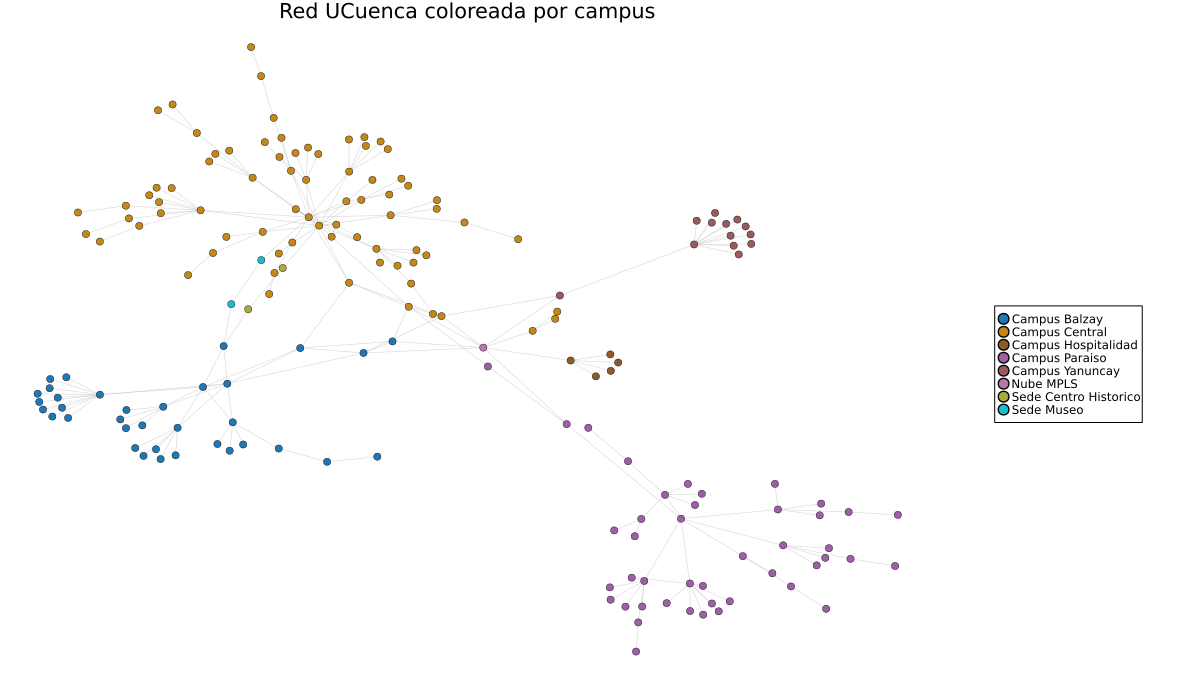
\includegraphics[width=\linewidth]{p2_red_por_campus.png}
\end{minipage}\hfill
\begin{minipage}{0.45\textwidth}\centering
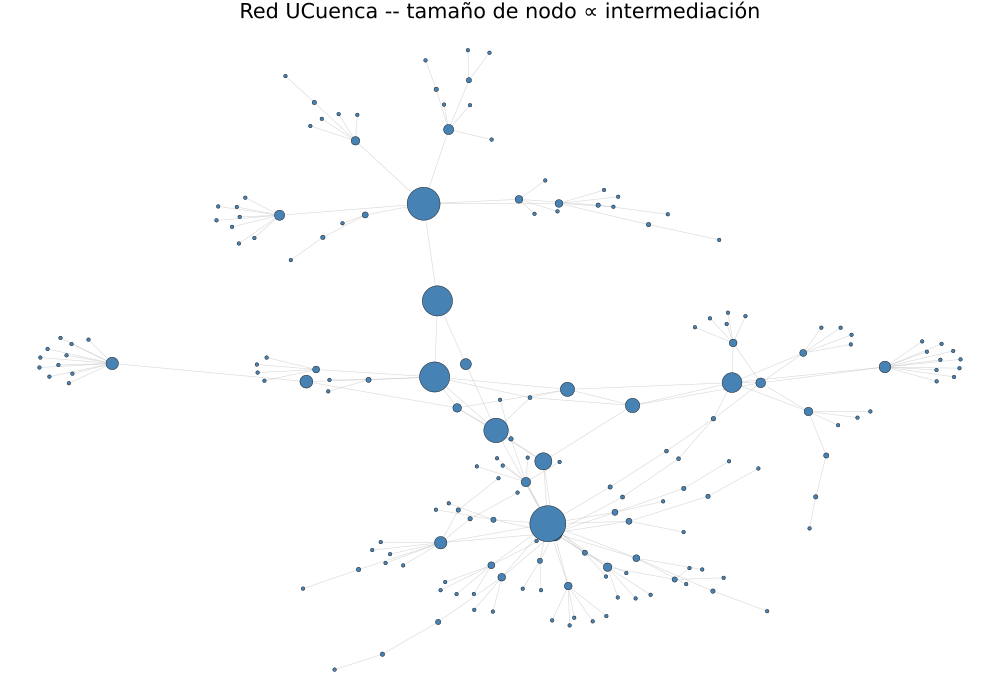
\includegraphics[width=\linewidth]{p2_red_por_intermediacion.png}
\end{minipage}
\caption{Dos visualizaciones de la misma red con el mismo \textit{layout} de resortes
(Fruchterman-Reingold, \code{NetworkLayout.jl}). \textbf{Izquierda:} color por campus; se
aprecian los siete bloques geográficos y el puñado de enlaces WAN que los cose.
\textbf{Derecha:} tamaño de nodo proporcional a la centralidad de intermediación; los pocos
nodos grandes son los \textit{core} y los \textit{routers} de interconexión, y confirman
visualmente el top-10 de la Tabla~\ref{tab:centralidades}.}
\label{fig:campus}
\end{figure}

Las dos figuras cuentan la misma historia desde ángulos distintos. La
Figura~\ref{fig:campus} muestra \textit{dónde} está cada cosa: siete islas de color
conectadas por muy pocos enlaces. La parte derecha muestra \textit{qué}
sostiene el conjunto: media docena de nodos desproporcionadamente grandes situados
justamente en las costuras entre islas. Superponer mentalmente ambas da el diagnóstico de
la red en una sola imagen.

\newpage
% ============================================================================
\section{Recorridos y comunidades (Fase 2)}

\textit{Unidad 2 del sílabo. Problemas P3 (BFS y DFS) y P4 (comunidades y modularidad).}

\subsection{P3 --- BFS y DFS sobre la red}

\subsubsection{Implementación y complejidad}

Ambos recorridos se implementaron desde cero sobre la lista de adyacencia del grafo:

\begin{itemize}[leftmargin=*,itemsep=1.5mm]
\item \textbf{BFS} con una \textbf{cola FIFO} (\code{Vector\{Int\}} con \code{popfirst!}).
Cada nodo se encola exactamente una vez y cada arista se examina a lo sumo dos veces ---una
desde cada extremo---, de modo que la complejidad es $O(V+E)$. Devuelve el orden de visita,
el vector de distancias en saltos y el vector de padres del árbol BFS.

\item \textbf{DFS} \textit{iterativo} con una \textbf{pila explícita} de pares
$(\text{nodo}, \text{índice del próximo vecino a probar})$. Se evitó deliberadamente la
recursión para no depender del límite de pila de Julia en grafos grandes. Misma complejidad
$O(V+E)$: la única diferencia con BFS es la estructura de datos (LIFO en vez de FIFO), y esa
diferencia es la que determina el orden de visita y, con él, el árbol de recorrido
resultante.
\end{itemize}

Ambas implementaciones se verificaron cruzadamente contra \code{Graphs.jl}: el BFS propio
reproduce exactamente el vector de distancias de \code{gdistances}, y el DFS propio visita
el mismo conjunto de nodos. La verificación es una aserción dentro del \textit{script}, de
modo que el pipeline aborta si alguna vez dejara de cumplirse.

\subsubsection{Perfil de profundidad desde el \textit{core} de Campus Central}

\begin{table}[H]
\centering
\caption{Nodos por distancia BFS desde el \textit{core} de Campus Central (\code{DATCC-2A-C2})}
\label{tab:perfilcore}
\small
\begin{adjustbox}{max width=\textwidth}
\begin{tabular}{lrrrrrrrrr}
\toprule
Distancia (saltos) & 0 & 1 & 2 & 3 & 4 & 5 & 6 & 7 & 8 \\
Nodos              & 1 & 16 & 48 & 19 & 9 & 41 & 7 & 29 & 7 \\
Acumulado          & 1 & 17 & 65 & 84 & 93 & 134 & 141 & 170 & 177 \\
\bottomrule
\end{tabular}
\end{adjustbox}
\end{table}

\textbf{¿La jerarquía declarada se refleja en las distancias medidas?} Solo parcialmente,
y la desviación es informativa. Si la jerarquía \textit{core}(0)--agregación(1)--acceso(2)
se cumpliera al pie de la letra, prácticamente todos los nodos deberían quedar a distancia
$\le 2$. \textbf{Solo 65 de 177 (36,7\,\%) lo hacen.} Los 16 nodos a distancia 1 son la
capa de agregación de Central más los \textit{routers} y \textit{firewalls} directamente
colgados del core, y los 48 a distancia 2 son sus equipos de acceso: hasta ahí, el informe
acierta.

El resto ---112 nodos, el 63\,\%--- forma una cola larga que llega hasta distancia 8. Esa
cola tiene dos causas distintas, y conviene no confundirlas: (i) \textbf{campus remotos}
(Paraíso, Yanuncay, Hospitalidad, las dos sedes) que solo alcanzan el \textit{core} de
Central atravesando la nube MPLS, lo que suma varios saltos WAN que un modelo de tres capas
no contempla porque describe \textit{un} campus, no la institución completa; y (ii)
\textbf{acceso indirecto} dentro de un mismo campus ---equipos de acceso colgados de otros
equipos de acceso, en cadena---, que es un anti-patrón de diseño y que la
Sección~\ref{sec:p8} volverá a encontrar como fragilidad. El salto abrupto de 9 nodos a
distancia 4 a 41 nodos a distancia 5 marca exactamente el punto en que el recorrido
«desemboca» en otro campus tras cruzar la WAN.

Repitiendo el BFS desde el otro \textit{switch} de core redundante (\code{DATCC-2A-C3}) el
perfil es idéntico, lo que confirma que los dos \textit{core} de Central son
intercambiables: cualquiera de los dos ve la red igual.

\subsubsection{Perfil desde la nube MPLS}

\begin{table}[H]
\centering
\caption{Nodos por distancia BFS desde \code{INTERNET-MPLS}}
\label{tab:perfilmpls}
\small
\begin{adjustbox}{max width=\textwidth}
\begin{tabular}{lrrrrrrr}
\toprule
Distancia (saltos) & 0 & 1 & 2 & 3 & 4 & 5 & 6 \\
Nodos              & 1 & 8 & 13 & 38 & 97 & 18 & 2 \\
Acumulado          & 1 & 9 & 22 & 60 & 157 & 175 & 177 \\
\bottomrule
\end{tabular}
\end{adjustbox}
\end{table}

El perfil desde la nube MPLS es mucho más compacto: máximo a distancia 6, con el 54,8\,\%
de la red concentrado a distancia exactamente 4 y el 88,7\,\% a distancia $\le 4$. La nube
MPLS es, por diseño, el punto más central de la topología inter-campus ---lo que ya
anticipaban sus valores de cercanía (primer puesto) e intermediación (cuarto puesto) en la
Tabla~\ref{tab:centralidades}.

\textbf{¿Qué campus quedan más «lejos» del resto de la institución?} Los dos nodos a
distancia 6 y la mayor parte de los 18 nodos a distancia 5 pertenecen a los campus que
necesitan más saltos internos después de aterrizar desde la WAN: los sub-laboratorios de
Paraíso y de Balzay conectados en cadena detrás de su switch de agregación. Los campus
pequeños (Hospitalidad, las sedes Museo y Centro Histórico) están, paradójicamente,
\textit{cerca} de la MPLS ---cuelgan casi directamente de ella--- pero eso no los hace
robustos: están cerca por un único enlace, y esa es exactamente la vulnerabilidad que la
Fase~5 propone corregir.

\subsubsection{Ciclos del grafo}

Con un árbol de expansión DFS de $n-1 = 176$ aristas, cada una de las $m-(n-1) = 33$
aristas restantes ---las «aristas de retroceso», no usadas por el árbol--- cierra
exactamente un \textbf{ciclo fundamental}. Ese número es el \textbf{número ciclomático}
$m - n + c = 209 - 177 + 1 = 33$ y \textit{no} depende del árbol elegido; sí depende del
árbol \textit{cuáles} aristas concretas se marcan como de retroceso.

\begin{table}[H]
\centering
\caption{Distribución de las 33 aristas generadoras de ciclo por ubicación (contando ambos extremos)}
\label{tab:ciclos}
\small
\begin{adjustbox}{max width=\textwidth}
\begin{tabular}{lrrrrrrr}
\toprule
Ubicación & Central & Balzay & Nube MPLS & Museo & C.\ Histórico & Paraíso & Yanuncay \\
Extremos  & 39 & 19 & 4 & 1 & 1 & 1 & 1 \\
\bottomrule
\end{tabular}
\end{adjustbox}
\end{table}

\textbf{¿Dónde están los ciclos?} Casi exclusivamente en las capas \textit{core} y
agregación de Campus Central y Campus Balzay. Doce de las 33 aristas de retroceso terminan
en \code{DATCC-2A-C2} ---son el segundo enlace de cada nodo de agregación de Central, el
que crea la ruta alternativa--- y tres en \code{DT-0A-C12}, el equivalente en Balzay. Los
cuatro restantes con extremo en la nube MPLS son los enlaces redundantes hacia los
\textit{routers} PE.

\textbf{La relación con los enlaces redundantes descritos en el informe es exacta:} la
ausencia de ciclos en una zona equivale a la ausencia de camino alternativo, es decir, a
una zona sin redundancia ---exactamente donde P1 localizó los puentes. Son el mismo
fenómeno visto desde dos algoritmos distintos. En efecto: ninguna de las 33 aristas de
retroceso puede ser puente (por definición, un puente no pertenece a ningún ciclo), y de las
176 aristas de árbol, 141 resultan ser puentes; las otras 35 son de árbol pero quedan
«cubiertas» por algún ciclo que las hace prescindibles. Paraíso y Yanuncay aportan un solo
extremo cada uno a la lista de ciclos: no tienen redundancia interna que crear ciclos, y por
eso son los campus que la Fase~5 prioriza.

\subsubsection{BFS, DFS y la tarea del técnico}

\textbf{¿Cuál de los dos recorridos modela mejor la visita física a todos los armarios de un
campus partiendo del \textit{core}?} \textbf{DFS, sin ambigüedad.} Un técnico que camina por
los edificios no puede «teletransportarse» entre ramas del árbol, que es exactamente lo que
hace BFS: visita todos los nodos a distancia 1, después todos los de distancia 2, saltando
de rama en rama y obligando a volver físicamente al \textit{core} entre visitas. DFS, en
cambio, avanza por una rama hasta el final antes de retroceder ---igual que recorrer un
pasillo o un edificio completo antes de pasar al siguiente. El orden que produce DFS es
directamente una ruta física razonable, en la que los retrocesos corresponden a caminar de
vuelta el mismo tramo; el orden por niveles de BFS, llevado a recorrido real, multiplicaría
los trayectos de ida y vuelta.

La matización honesta es que DFS tampoco es óptimo: el problema exacto ---visitar todos los
nodos minimizando la distancia caminada--- es una variante del problema del cartero chino
sobre el árbol de expansión, y DFS es solo una heurística razonable para él. Pero entre las
dos opciones que el enunciado plantea, la diferencia no es de matiz: es la diferencia entre
una ruta caminable y una que no lo es.

\subsection{P4 --- Comunidades y modularidad}

\subsubsection{Louvain y estabilidad}

Se implementó Louvain completo desde cero (Blondel et al., 2008): fase de movimiento local
voraz, en la que cada nodo se reasigna a la comunidad vecina que maximiza la ganancia de
modularidad $\Delta Q$, alternada con una fase de agregación en la que cada comunidad
colapsa a un super-nodo, hasta que agregar ya no reduce el número de super-nodos. Sobre la
red UCuenca encuentra \textbf{22 comunidades con $Q = 0{,}7504$}, una modularidad muy alta,
característica de una red con bloques jerárquicos bien separados.

\begin{table}[H]
\centering
\caption{Estabilidad de Louvain en cinco semillas distintas (P4.1)}
\label{tab:louvain}
\small
\begin{adjustbox}{max width=\textwidth}
\begin{tabular}{rrrr}
\toprule
\textbf{Semilla} & \textbf{Comunidades} & \textbf{$Q$} & \textbf{NMI vs.\ corrida de referencia (semilla 1217)} \\
\midrule
1    & 21 & 0,7508 & 0,9565 \\
2    & 22 & 0,7497 & 0,9792 \\
3    & 22 & 0,7504 & 0,9857 \\
42   & 22 & 0,7357 & 0,9279 \\
2024 & 22 & 0,7497 & 0,9744 \\
\bottomrule
\end{tabular}
\end{adjustbox}
\end{table}

El resultado es \textbf{estable}: el número de comunidades varía apenas entre 21 y 22, la
modularidad entre 0,736 y 0,751, y la información mutua normalizada contra la corrida de
referencia nunca baja de 0,928. La variabilidad residual proviene del orden aleatorio en que
la fase local recorre los nodos, y afecta solo a la asignación de unos pocos nodos frontera
---no a la estructura de bloques.

\subsubsection{Comparación con la partición por campus}

\begin{table}[H]
\centering
\caption{Concordancia entre la partición de Louvain y la partición «natural» por \code{campus}}
\label{tab:nmiari}
\small
\begin{adjustbox}{max width=\textwidth}
\begin{tabular}{lcc}
\toprule
\textbf{Comparación} & \textbf{NMI} & \textbf{ARI} \\
\midrule
Louvain vs.\ partición por campus            & 0,584 & 0,190 \\
$k$-means espectral ($K=22$) vs.\ Louvain    & 0,834 & 0,372 \\
\bottomrule
\end{tabular}
\end{adjustbox}
\end{table}

La matriz de confusión comunidad $\times$ campus se presenta completa en la
Tabla~\ref{tab:confusion} (fuente: \code{p4\_matriz\_confusion\_comunidad\_campus.csv}). Es
casi bloque-diagonal: \textbf{Louvain no mezcla campus entre sí}, pero \textbf{sí subdivide
cada campus grande en varias comunidades}. Campus Central se reparte en once comunidades,
Balzay en cuatro y Paraíso en cinco. De ahí la aparente contradicción de los dos índices: el
NMI es moderado (0,584) porque la partición de Louvain \textit{refina} la de campus y
comparte con ella mucha información; el ARI es bajo (0,190) porque penaliza específicamente
la sobre-partición, y aquí la hay por construcción. Los dos índices no se contradicen: miden
cosas distintas y ambos son correctos.

\begin{table}[H]
\centering
\caption{Matriz de confusión comunidad de Louvain $\times$ campus declarado (22 comunidades $\times$ 8 campus); celdas en blanco = 0 (P4.3)}
\label{tab:confusion}
\scriptsize
\begin{adjustbox}{max width=\textwidth}
\begin{tabular}{rcccccccc}
\toprule
\textbf{Com.} & \textbf{Balzay} & \textbf{Central} & \textbf{Hospit.} & \textbf{Paraíso} & \textbf{Yanuncay} & \textbf{Nube MPLS} & \textbf{C.\ Histórico} & \textbf{Museo} \\
\midrule
1  &    & 4  &   &   &   &   &   &   \\
2  &    &    &   &   & 12 &   &   &   \\
3  & 11 &    &   &   &   &   &   &   \\
4  & 7  &    &   &   &   &   &   &   \\
5  &    & 6  &   &   &   &   &   &   \\
6  &    & 12 &   &   &   &   &   &   \\
7  &    & 5  &   &   &   &   &   &   \\
8  &    & 8  &   &   &   &   &   &   \\
9  &    & 3  &   &   &   &   &   &   \\
10 &    &    &   & 9 &   &   &   &   \\
11 &    &    &   & 6 &   &   &   &   \\
12 &    &    &   & 9 &   &   &   &   \\
13 &    &    &   & 7 &   &   &   &   \\
14 &    &    & 5 &   &   &   &   &   \\
15 & 3  & 3  &   & 2 & 1 & 1 &   &   \\
16 &    & 6  &   &   &   &   &   &   \\
17 &    & 4  &   &   &   &   &   &   \\
18 &    & 5  &   &   &   &   &   &   \\
19 & 14 &    &   &   &   &   &   & 2 \\
20 &    & 12 &   &   &   &   & 2 &   \\
21 &    &    &   & 11 &   &   &   &   \\
22 &    & 7  &   &   &   &   &   &   \\
\bottomrule
\end{tabular}
\end{adjustbox}
\end{table}

La comunidad 15 es la única con dispersión real entre campus (Balzay, Central, Paraíso,
Yanuncay y Nube MPLS a la vez) y coincide, como era de esperar, con el grupo donde se
concentran los nodos discrepantes de la Tabla~\ref{tab:discrepantes}: son los equipos WAN e
\textit{interconexión} de alta centralidad que Louvain agrupa por rol de tránsito compartido
en vez de por campus declarado. Todas las demás comunidades caen íntegramente dentro de un
único campus, lo que hace visualmente evidente el patrón «bloque-diagonal, pero
sobre-particionado» descrito arriba.

\textbf{Los nodos donde ambas particiones discrepan.} Solo \textbf{11 de 177 nodos} quedan
en una comunidad dominada por un campus distinto al propio, y no son un conjunto arbitrario:

\begin{table}[H]
\centering
\caption{Nodos cuya comunidad de Louvain está dominada por un campus distinto al declarado (P4.3)}
\label{tab:discrepantes}
\small
\begin{adjustbox}{max width=\textwidth}
\begin{tabular}{lll}
\toprule
\textbf{Equipo} & \textbf{Campus declarado} & \textbf{Campus dominante de su comunidad} \\
\midrule
INTERNET-MPLS                  & Nube MPLS             & Campus Balzay \\
FORTIGATE-1800F-CENTRAL        & Campus Central        & Campus Balzay \\
PE1-CENTRAL                    & Campus Central        & Campus Balzay \\
PE2-CENTRAL                    & Campus Central        & Campus Balzay \\
ROUTER-CAMPUS-HUAYNA-CAPAC     & Campus Paraíso        & Campus Balzay \\
ROUTER-CAMPUS-PARAISO          & Campus Paraíso        & Campus Balzay \\
ROUTER-CAMPUS-YANUNCAY         & Campus Yanuncay       & Campus Balzay \\
ROUTER-CAMPUS-MUSEO            & Sede Museo            & Campus Balzay \\
SW-ARUBA-MUSEO                 & Sede Museo            & Campus Balzay \\
ROUTER-CAMPUS-CENTRO-HISTORICO & Sede Centro Histórico & Campus Central \\
SW-ARUBA-CENTRO-HISTORICO      & Sede Centro Histórico & Campus Central \\
\bottomrule
\end{tabular}
\end{adjustbox}
\end{table}

\textbf{¿Qué significa, en términos de ingeniería de red, que un equipo etiquetado en un
campus quede agrupado con otro?} Que su conectividad real lo liga más al otro bloque que al
propio. Los once discrepantes son, casi sin excepción, equipos de \textbf{WAN e
interconexión}: los dos \textit{routers} PE de Central, el \textit{firewall} perimetral, la
nube MPLS y los \textit{routers} de campus de Paraíso, Yanuncay, Museo y Centro Histórico.
Louvain los agrupa todos juntos ---en la comunidad que también contiene equipos de Balzay---
porque forman un \textbf{núcleo WAN} funcionalmente propio, un bloque que existe en la
topología pero que la etiqueta \code{campus} (que es geográfica) no puede expresar. El
resultado no es un error del algoritmo: es una segunda partición legítima, ortogonal a la
geográfica, que el administrador de red reconocería inmediatamente como «la capa WAN».

Las dos sedes pequeñas (Museo y Centro Histórico, dos equipos cada una) se absorben enteras
en la comunidad de su punto de anclaje ---no tienen masa suficiente para formar comunidad
propia. Ese comportamiento anticipa exactamente la limitación que se discute a continuación.

\subsubsection{$k$-means sobre el espectro del laplaciano}

Se aplicó $k$-means (implementación desde cero con inicialización \textit{k-means++},
reutilizada de \code{codigo\_referencia/kmeans/}) sobre una representación vectorial de los
nodos: las $K=22$ primeras componentes no triviales del espectro del laplaciano, omitiendo
el autovector constante asociado al autovalor $\approx 0$, que no separa nada. El resultado
coincide parcialmente con Louvain (NMI $=0{,}834$, ARI $=0{,}372$).

\textbf{¿Por qué un método basado en distancias euclídeas puede o no ser adecuado para un
grafo?} La coincidencia parcial es el resultado esperable, no un fallo. El espacio espectral
usa distancia \textbf{euclídea} entre coordenadas derivadas del laplaciano; Louvain optimiza
directamente la \textbf{modularidad} sobre la topología (conteo de aristas), sin necesitar
ninguna noción de distancia entre nodos. Cuando el grafo es muy disperso y jerárquico como
este (grado medio 2,36), los primeros autovectores capturan sobre todo las ramas más grandes
del árbol de expansión ---los cortes que separan campus enteros--- y no necesariamente los
mismos bloques que Louvain identifica por densidad local de aristas. La ventaja del método
espectral es que produce una representación vectorial reutilizable (por ejemplo, para
alimentar otros modelos); su desventaja es que impone una geometría euclídea que el grafo no
tiene, y que exige fijar $K$ de antemano, cosa que Louvain no necesita.

\subsubsection{Límite de resolución de la modularidad}

La modularidad tiene un límite de resolución conocido (Fortunato \& Barthélemy, 2007): con
$m = 209$ aristas, dos comunidades solo se separan si la suma de sus grados internos supera
aproximadamente $\sqrt{2m} = \sqrt{418} \approx 20{,}4$.

\textbf{¿Podría Louvain estar fusionando bloques que un administrador de red consideraría
separados? Sí, y hay evidencia concreta.} Las 22 comunidades tienen entre 3 y 16 nodos
(mediana 7), y \textbf{tres de ellas tienen 4 nodos o menos}: están claramente por debajo
del umbral de resolución. La evidencia más nítida son las dos sedes pequeñas: Museo (2
equipos) y Centro Histórico (2 equipos) \textbf{no aparecen como comunidades propias} en la
partición ---quedan absorbidas en la comunidad de Balzay y de Central respectivamente
(Tabla~\ref{tab:discrepantes})--- pese a que un administrador de red las trata sin duda como
dominios administrativos separados, con su propia VLAN y su propio contrato de enlace. La
modularidad no puede «verlas» porque la suma de sus grados internos es demasiado pequeña
frente a $\sqrt{2m}$. La corrección estándar sería usar modularidad con parámetro de
resolución $\gamma > 1$ o un método que no dependa de una escala global, como el
\textit{stochastic block model}; no se aplica aquí porque excede el alcance del enunciado,
pero la limitación queda documentada.

% ============================================================================
\section{Optimización en redes (Fase 3)}

\textit{Unidad 3 del sílabo. Problemas P5 (caminos más cortos), P6 (flujo máximo y corte
mínimo) y P7 (localización de instalaciones).}

\subsection{P5 --- Caminos más cortos}

\subsubsection{Los tres modelos de peso y su justificación}

Antes de aplicar cualquier algoritmo de camino más corto hay que decidir \textbf{qué se
minimiza}. Se implementaron y compararon los tres modelos propuestos por el enunciado:

\begin{align}
w_{\text{saltos}}(u,v)   &= 1 \\
w_{\text{latencia}}(u,v) &= \alpha + \frac{\beta}{c(u,v)}, \qquad \alpha = 0{,}05\ \text{ms},\ \beta = 12\ \text{Mbit} \\
w_{\text{carga}}(u,v)    &= \frac{b(u,v)}{c(u,v)}
\end{align}

La elección de las constantes se justifica físicamente y no por conveniencia numérica:
$\alpha = 0{,}05$~ms representa la latencia fija de propagación más conmutación por salto,
razonable a escala de campus (decenas de kilómetros a lo sumo, más el retardo de un switch o
router L2--L3); $\beta = 12$~Mbit corresponde al tamaño de una trama Ethernet típica
($\approx 1500$~B $\approx 12$~kbit), de modo que $\beta/c$ da directamente el tiempo de
serialización en milisegundos cuando $c$ está en Mbps. Con esos valores, un enlace de
10~Gbps aporta $0{,}0512$~ms y uno de 1~Gbps aporta $0{,}062$~ms: la diferencia es pequeña
pero sistemática, y basta para cambiar rutas cuando se acumula sobre once saltos.

\subsubsection{Dijkstra y Floyd-Warshall: implementación y verificación}

\textbf{Dijkstra} se implementó con una cola de prioridad propia ---un montículo binario
mínimo con \code{push!}/\code{pop!} en $O(\log n)$---, dando complejidad
$O((V+E)\log V)$ por fuente. \textbf{Floyd-Warshall} se implementó en su forma clásica de
tres bucles anidados sobre la matriz densa de pesos, complejidad $O(V^3)$.

La verificación exigida por el enunciado se hizo sobre \textbf{20 pares de nodos elegidos al
azar} y para los \textbf{tres modelos de peso}: en los 60 casos la distancia de Dijkstra
coincide con la entrada correspondiente de la matriz de Floyd-Warshall con tolerancia
$10^{-9}$. La verificación es una aserción del \textit{script}, no una comprobación manual.

\subsubsection{Comparación empírica de tiempos}

\begin{table}[H]
\centering
\caption{Dijkstra (una fuente) frente a Floyd-Warshall sobre subredes de tamaño creciente,
construidas tomando los primeros $n$ nodos del orden BFS desde el \textit{core}}
\label{tab:tiempos}
\small
\begin{adjustbox}{max width=\textwidth}
\begin{tabular}{rrrr}
\toprule
$n$ & \textbf{Floyd-Warshall (s)} & \textbf{Dijkstra, 1 fuente (s)} & \textbf{Fuentes de equilibrio} \\
\midrule
20  & 0,000009  & 0,0000091 & 1 \\
40  & 0,0000714 & 0,0000062 & 12 \\
60  & 0,000188  & 0,0000033 & 57 \\
80  & 0,000427  & 0,0000057 & 75 \\
100 & 0,000772  & 0,0000069 & 112 \\
130 & 0,001628  & 0,0000078 & 209 \\
177 & 0,004082  & 0,0000427 & 96 \\
\bottomrule
\end{tabular}
\end{adjustbox}
\end{table}

\textbf{¿A partir de qué tamaño, y para cuántos pares consultados, conviene cada uno?} La
columna «fuentes de equilibrio» responde exactamente esa pregunta: es el número de corridas
de Dijkstra que cuestan lo mismo que \textit{una} corrida completa de Floyd-Warshall. Por
debajo de ese número de fuentes que realmente interesan, conviene Dijkstra repetido; por
encima, conviene una sola pasada de Floyd-Warshall, que da todos los pares de una vez.

El punto de equilibrio crece con $n$ de $\sim 1$ a $\sim 200$ fuentes, que es justamente lo
que predice la teoría: el cociente entre $O(V^3)$ y $O((V+E)\log V)$ crece
aproximadamente como $V^2/\log V$. Las curvas medidas siguen esa tendencia con la dispersión
propia de tiempos de ejecución del orden de microsegundos, dominados por efectos de caché y
de asignación de memoria más que por el conteo de operaciones ---la anomalía visible en la
última fila ($n=177$, donde la medición de Dijkstra sube un orden de magnitud por incluir el
coste de asignación del montículo sobre el grafo completo) es de esa naturaleza. Para esta
red la conclusión práctica es clara: como el análisis necesita la matriz \textit{completa}
de distancias (para cercanía, para $p$-mediana y para $p$-centro), Floyd-Warshall es la
elección correcta, y en $n = 177$ tarda 4~ms.

\subsubsection{Cercanía bajo cada modelo de peso}

\begin{table}[H]
\centering
\caption{Top-10 por cercanía bajo los tres modelos de peso, lado a lado (P5.3)}
\label{tab:cercania}
\scriptsize
\setlength{\tabcolsep}{2.8pt}
\begin{adjustbox}{max width=\textwidth}
\begin{tabular}{r|lr|lr|lr}
\toprule
\# & \textbf{$w_{\text{saltos}}$} & Cerc. & \textbf{$w_{\text{latencia}}$} & Cerc. & \textbf{$w_{\text{carga}}$} & Cerc. \\
\midrule
1  & INTERNET-MPLS            & 0,001567 & INTERNET-MPLS            & 0,02878 & AGRPRI-1A-D10        & 0,05132 \\
2  & DATCC-2A-C3              & 0,001524 & PE2-CENTRAL              & 0,02790 & CC-AETUC-D30         & 0,05132 \\
3  & PE2-CENTRAL              & 0,001515 & DATCC-2A-C3              & 0,02775 & CC-ARQUITECTURA-D107 & 0,05132 \\
4  & FORTIGATE-1800F-CENTRAL  & 0,001475 & FORTIGATE-1800F-CENTRAL  & 0,02689 & CC-BIBLIOTECA-D112   & 0,05132 \\
5  & PE1-CENTRAL              & 0,001456 & PE1-CENTRAL              & 0,02686 & CC-BLOQUE-IQ         & 0,05132 \\
6  & PE1-BALZAY               & 0,001427 & PE1-BALZAY               & 0,02634 & CC-ECONOMIA-D51      & 0,05132 \\
7  & DATCC-2A-C2              & 0,001406 & DATCC-2A-C2              & 0,02571 & CC-FILOSOFIA-A-D108  & 0,05132 \\
8  & ROUTER-HUAYNA-CAPAC      & 0,001376 & ROUTER-HUAYNA-CAPAC      & 0,02545 & CC-FILOSOFIA-B-D111  & 0,05132 \\
9  & FORTIGATE-1800F-BALZAY   & 0,001368 & PE2-BALZAY               & 0,02507 & CC-MONJAS-D126       & 0,05132 \\
10 & PE2-BALZAY               & 0,001355 & FORTIGATE-1800F-BALZAY   & 0,02477 & CC-PROMAS-D31        & 0,05132 \\
\bottomrule
\end{tabular}
\end{adjustbox}
\end{table}

\textbf{¿Cambia el ranking según el peso elegido?} Depende radicalmente del peso:

\begin{itemize}[leftmargin=*,itemsep=1.5mm]
\item $w_{\text{saltos}}$ y $w_{\text{latencia}}$ coinciden en \textbf{10 de 10} nodos
(con dos intercambios menores de posición). Era esperable: con $\alpha \gg$ la variación de
$\beta/c$, el modelo de latencia es una perturbación pequeña del de saltos. El resultado
tiene valor de \textit{control}: confirma que el modelo de latencia está bien calibrado y no
produce rutas absurdas.

\item $w_{\text{carga}}$ cambia el ranking \textbf{por completo (0 de 10 de coincidencia)} y
muestra un empate exacto de 51 nodos con idéntica cercanía. La causa está en los datos:
\textbf{51 de las 209 aristas tienen tráfico medido o asumido igual a 0~Mbps} y, por tanto,
peso \textit{exactamente} 0 bajo este modelo. Muchos equipos de acceso quedan a distancia 0
de su switch, y la cercanía agregada se colapsa en empates. \textbf{Esto no es un error de
cálculo: es una propiedad real del modelo}, que mide congestión y no topología. Un enlace
sin tráfico registrado es, para $w_{\text{carga}}$, un enlace «gratis», y eso es
conceptualmente correcto ---aunque haga que la cercanía deje de ser una medida útil de
posición estructural.
\end{itemize}

\subsubsection{El par de equipos de acceso más distante}

\begin{table}[H]
\centering
\caption{Par de equipos de acceso más distante bajo cada modelo de peso (P5.4)}
\label{tab:pardistante}
\small
\begin{adjustbox}{max width=\textwidth}
\begin{tabular}{llr}
\toprule
\textbf{Modelo} & \textbf{Par más distante} & \textbf{Distancia} \\
\midrule
$w_{\text{saltos}}$   & ENF-2B-A122 $\leftrightarrow$ POST-2A-A66   & 11 saltos \\
$w_{\text{latencia}}$ & POST-2A-A66 $\leftrightarrow$ QUIN-1A-A128  & 0,639 ms \\
$w_{\text{carga}}$    & ECOK1-1A-A102 $\leftrightarrow$ INV-1B-A162 & 0,710 \\
\bottomrule
\end{tabular}
\end{adjustbox}
\end{table}

La ruta salto a salto bajo $w_{\text{saltos}}$ ilustra perfectamente la topología de la
institución:

\begin{center}\small
\code{ENF-2B-A122} $\to$ \code{ENF-2B-A22} $\to$ \code{CP-ENFERMERIA-D1} $\to$
\code{CPAR-C10} $\to$ \code{ROUTER-CAMPUS-HUAYNA-CAPAC} $\to$ \code{INTERNET-MPLS} $\to$\\
\code{PE2-CENTRAL} $\to$ \code{DATCC-2A-C3} $\to$ \code{CC-FILOSOFIA-A-D108} $\to$
\code{POST-1A-A64} $\to$ \code{POST-1A-A65} $\to$ \code{POST-2A-A66}
\end{center}

Once saltos para ir de un aula de Enfermería (Paraíso) a un aula de Posgrado (Central):
sube por su switch de acceso y de agregación, atraviesa el \textit{único} core de Paraíso,
sale por el \textit{router} de campus, cruza la nube MPLS, entra por el PE de Central, baja
al core, a agregación y encadena \textit{dos} equipos de acceso más. La ruta pasa
obligatoriamente por \code{CPAR-C10} y por \code{ROUTER-CAMPUS-HUAYNA-CAPAC}, los dos nodos
que P6 y P10 identificarán como los más críticos de Paraíso.

\textbf{El modelo de peso sí cambia cuál es el par «más lejano»}: bajo
$w_{\text{latencia}}$ la ruta más costosa deja de ser la que cruza Paraíso y pasa a ser la
que atraviesa Balzay (\code{POST-2A-A66} $\leftrightarrow$ \code{QUIN-1A-A128}, también de
once saltos), porque penaliza más los saltos de baja capacidad que los de alta ---y la ruta
por Balzay acumula más tramos de 1~Gbps.

\subsubsection{Pesos negativos y protocolos reales}

\textbf{Ninguno de los tres modelos puede producir un peso negativo:}
$w_{\text{saltos}} = 1$ siempre; $w_{\text{latencia}} = \alpha + \beta/c$ con
$\alpha, \beta > 0$ y $c > 0$ (la capacidad estimada es siempre estrictamente positiva); y
$w_{\text{carga}} = b/c$ con $b, c \ge 0$. Dijkstra es, por tanto, válido en los tres casos
sin necesidad de recurrir a Bellman-Ford. La única excepción del proyecto es el algoritmo de
flujo de costo mínimo de la Sección~\ref{sec:mincost}, donde la \textit{red residual} sí
genera arcos de costo negativo y por eso allí se usa Bellman-Ford deliberadamente.

\textbf{¿Qué modelo usaría un protocolo real y qué ocurriría si el peso dependiera del
tráfico instantáneo?} OSPF e IS-IS usan en la práctica un costo \textbf{estático},
típicamente proporcional al inverso del ancho de banda nominal ---muy parecido a
$w_{\text{latencia}}$ con el término de tráfico fuera de la fórmula---, y \textbf{no} un
costo que dependa del tráfico instantáneo como $w_{\text{carga}}$. La razón es un modo de
falla concreto: si el peso dependiera de la carga en tiempo real, cada cambio de tráfico
dispararía un recálculo de rutas (inundación de LSA / actualización de estado de enlace) y
el tráfico que huye de un enlace congestionado podría sobrecargar la ruta alternativa,
haciendo que \textit{esa} se vuelva «cara» y el tráfico regrese. El resultado es
\textbf{oscilación de rutas} (\textit{route flapping}) e inestabilidad, un problema
documentado desde los primeros diseños de enrutamiento adaptativo de ARPANET. El costo
estático sacrifica optimalidad instantánea a cambio de convergencia garantizada, y es la
decisión de ingeniería correcta.

\subsection{P6 --- Flujo máximo y corte mínimo}
\label{sec:p6}

\subsubsection{Estimación de la función de capacidad}
\label{sec:capacidad}

La capacidad nominal solo está documentada en 28 de las 209 aristas ---todas del diagrama
MPLS. Las 181 restantes se estimaron con reglas explícitas, y el supuesto aplicado se
registra \textbf{arista por arista} en \code{p6\_capacidad\_estimada.csv} para que cualquier
lector pueda auditarlo:

\begin{table}[H]
\centering
\caption{Reglas de estimación de capacidad y número de aristas afectadas (P6.1)}
\label{tab:capacidad}
\small
\begin{adjustbox}{max width=\textwidth}
\begin{tabular}{p{9.5cm}rr}
\toprule
\textbf{Regla} & \textbf{Aristas} & \textbf{Capacidad} \\
\midrule
Documentada explícitamente en el diagrama MPLS & 28 & 1--20 Gbps \\
Troncal \textit{core}--agregación: el informe declara 10 Gbps (cap.~2.1) & 40 & 10 Gbps \\
\code{rol} $\in$ \{\code{wan}, \code{inferido}\}: por analogía con los enlaces MPLS documentados & 7 & 10 Gbps \\
Agregación--acceso o \textit{core}--acceso: \textit{uplink} Ethernet estándar & 111 & 1 Gbps \\
Otros casos (\textit{firewalls} de interconexión, \textit{core}--\textit{core}): por defecto & 23 & 1 Gbps \\
\midrule
\textbf{Total} & \textbf{209} & \\
\bottomrule
\end{tabular}
\end{adjustbox}
\end{table}

La distribución resultante es 139 aristas a 1~Gbps, 68 a 10~Gbps y 2 a 20~Gbps. La regla
más discutible del conjunto es la cuarta ---1~Gbps para los 111 \textit{uplinks} de
acceso---, porque no está declarada por el informe y afecta a más de la mitad de las
aristas; se señala como tal.

\begin{clave}
\textbf{Hallazgo original (inconsistencia detectada en los datos).} El enlace
\code{DATCC-2A-C2}--\code{DATCC-2A-C3}, que une los dos \textit{core} de Campus Central,
registra un tráfico medido de \textbf{1\,890~Mbps} sobre una capacidad \textit{estimada} de
1\,000~Mbps: una utilización $b/c = 1{,}89 > 1$, físicamente imposible. La causa es que ese
enlace cae en la quinta regla (\textit{core}--\textit{core} no cubierto por ninguna regla
específica) y recibe el valor por defecto de 1~Gbps. La medición demuestra que la
estimación es incorrecta: ese enlace opera necesariamente a 10~Gbps o más. Es el único de
las 209 aristas con $b/c > 1$, lo que a la vez valida el resto de las reglas y aísla el
único punto donde fallan. Corregirlo no altera ningún resultado de flujo de este informe
(el enlace no pertenece a ningún corte mínimo), pero sí sería obligatorio en cualquier
extensión del análisis, y se documenta aquí como recomendación de mejora del conjunto de
datos.
\end{clave}

\subsubsection{Flujo máximo por campus}

Se modeló, para cada campus, el problema «todo el tráfico del campus sale hacia Internet»:
se añade una \textbf{super-fuente} conectada a todos los equipos de acceso del campus con
capacidad artificialmente enorme (200\,000~Mbps, muy por encima de cualquier capacidad
real, para que nunca sea el cuello de botella), y se toma como sumidero
\code{INTERNET-MPLS}. Se resolvió con \textbf{Ford-Fulkerson} (búsqueda DFS) y con
\textbf{Edmonds-Karp} (búsqueda BFS), reutilizando las implementaciones de
\code{codigo\_referencia/}. Ambos devuelven \textit{el mismo} flujo máximo en los siete
casos, como exige el teorema.

\begin{table}[H]
\centering
\caption{Flujo máximo por campus hacia \code{INTERNET-MPLS} y corte mínimo asociado (P6.2--P6.3)}
\label{tab:flujo}
\small
\begin{adjustbox}{max width=\textwidth}
\begin{tabular}{lrrrrrcc}
\toprule
\textbf{Campus} & \textbf{Nodos de acceso} & \textbf{Flujo máx.\ (Mbps)} & \textbf{Aristas del corte} & \textbf{Cap.\ del corte} & \textbf{Iter.\ FF / EK} & \textbf{Long.\ caminos FF} & \textbf{Long.\ caminos EK} \\
\midrule
Campus Central        & 56 & 44\,000 &  7 & 44\,000 & 44 / 44 & 3--13 & 3--12 \\
Campus Balzay         & 24 & 23\,000 & 23 & 23\,000 & 23 / 23 & 5--11 & 5--7 \\
Sede Museo            &  1 & 11\,000 &  2 & 11\,000 &  3 / 3 & 5--8 & 5--6 \\
Sede Centro Histórico &  1 & 11\,000 &  2 & 11\,000 &  4 / 2 & 5--10 & 4--6 \\
Campus Yanuncay       & 11 & 10\,000 &  1 & 10\,000 & 10 / 10 & 4--4 & 4--4 \\
Campus Hospitalidad   &  4 &  4\,000 &  4 &  4\,000 &  4 / 4 & 3--3 & 3--3 \\
\textbf{Campus Paraíso} & \textbf{35} & \textbf{1\,000} & \textbf{1} & \textbf{1\,000} & \textbf{1 / 1} & \textbf{5--5} & \textbf{5--5} \\
\bottomrule
\end{tabular}
\end{adjustbox}
\end{table}

\textbf{Verificación manual del teorema max-flow / min-cut.} En los siete casos, la suma de
las capacidades de las aristas del corte coincide \textit{exactamente} con el valor del
flujo máximo ---la verificación es una aserción del \textit{script}, que aborta si falla. El
caso de Paraíso puede comprobarse a mano en una línea: el corte consta de una única arista,
\code{CPAR-C10}--\code{ROUTER-CAMPUS-HUAYNA-CAPAC}, de capacidad 1\,000~Mbps, y el flujo
máximo es 1\,000~Mbps.

\textbf{Longitudes de los caminos aumentantes.} Las dos últimas columnas reportan, para cada
campus, el rango (mínimo--máximo, en saltos) de las longitudes de \textit{todos} los
caminos aumentantes usados a lo largo de la ejecución ---no solo su número, que ya estaba en
la columna de iteraciones. Dos lecturas se desprenden directamente de estos rangos. Primero,
\textbf{Edmonds-Karp nunca usa caminos más largos que Ford-Fulkerson y casi siempre usa
caminos más cortos o iguales}: el máximo de EK es menor o igual que el de FF en los siete
casos (p.~ej.\ Central: 12 contra 13; Balzay: 7 contra 11), consistente con que EK busca
explícitamente el camino \textit{más corto} disponible en cada iteración, mientras que FF
(DFS) puede tomar rutas más largas y menos eficientes antes de agotar la red residual.
Segundo, y más fuerte: \textbf{la secuencia completa de longitudes de EK es siempre no
decreciente}, la propiedad que garantiza su cota $O(V\!\cdot\!E)$ (Cormen et al., 2009,
cap.~26); el \textit{script} lo verifica con una aserción explícita
(\code{issorted(longitudes\_ek)}) que se cumple en los siete campus. El caso de Sede Centro
Histórico lo ilustra en una corrida de solo dos iteraciones: EK usa longitudes
$4 \to 6$ (crece), mientras que FF, sin esa garantía, usa $10 \to 6 \to 5 \to 8$ en sus
cuatro iteraciones ---sube y baja sin ningún patrón, y por eso necesita el doble de
iteraciones para llegar al mismo flujo máximo.

\textbf{El resultado es contundente: Paraíso, con 35 equipos de acceso ---más que Yanuncay
y Hospitalidad juntos---, tiene el flujo máximo más bajo de toda la institución}, cuarenta y
cuatro veces menor que el de Central y once veces menor que el de Yanuncay, que tiene un
tercio de sus equipos. Es la confirmación cuantitativa, y por una vía completamente
independiente, del hallazgo estructural de la Sección~\ref{sec:contraste}.

\subsubsection{Interpretación de los cortes mínimos}

\textbf{¿Qué enlaces físicos concretos componen cada corte? ¿Coinciden con los puentes de
P1? ¿Con lo que el informe describe como no redundante?} Las tres respuestas son
afirmativas y se refuerzan mutuamente:

\begin{table}[H]
\centering
\caption{Composición de los cortes mínimos más ilustrativos}
\label{tab:cortes}
\small
\begin{adjustbox}{max width=\textwidth}
\begin{tabular}{llr@{\hspace{4mm}}c}
\toprule
\textbf{Campus} & \textbf{Arista del corte} & \textbf{Cap.\ (Mbps)} & \textbf{¿Es puente de P1?} \\
\midrule
Paraíso     & CPAR-C10 -- ROUTER-CAMPUS-HUAYNA-CAPAC & 1\,000 & \textbf{sí} \\
Yanuncay    & AGRPRI-1A-D10 -- ROUTER-CAMPUS-YANUNCAY & 10\,000 & \textbf{sí} \\
Hospitalidad& HOS-0A-A10/A13/A11/A12 -- HOS-0A-D05 (4 aristas) & $4\times 1\,000$ & \textbf{sí} \\
Central     & DATCC-2A-C3 -- PE2-CENTRAL & 20\,000 & no \\
Central     & DATCC-2A-C2/C3 -- FORTIGATE-1800F-CENTRAL & $2\times 10\,000$ & no \\
Central     & CCJ-1A-A10/A11 -- CCJ-CJURIDICO-D4 & $2\times 1\,000$ & \textbf{sí} \\
\bottomrule
\end{tabular}
\end{adjustbox}
\end{table}

La lectura operativa es directa. Cuando una arista del corte mínimo \textit{también} aparece
en la lista de puentes de P1, la falla de \textbf{ese único enlace} reduce a cero el flujo
de salida del campus: el cuello de botella físico y el punto de fragilidad topológica
coinciden. Ese es exactamente el caso de Paraíso, Yanuncay y Hospitalidad. En Campus
Central, en cambio, el corte está formado por siete aristas de alta capacidad, ninguna de
las cuales es puente por sí sola (salvo el sub-bloque del Consultorio Jurídico): perder una
degrada el caudal pero no desconecta nada. La diferencia entre los dos escenarios es
precisamente la redundancia que el informe atribuía a ambos.

\subsubsection{Flujo de costo mínimo}
\label{sec:mincost}

Se formuló un problema de flujo de costo mínimo sobre la misma red asignando un costo por
unidad de flujo a cada arista: \textbf{1 por salto} en el caso general y \textbf{5 si el
enlace tiene \code{rol=respaldo}}, para penalizar el uso de rutas de respaldo salvo que sean
estrictamente necesarias. Se impuso una demanda fija simultánea desde dos campus
---\textbf{Balzay (11\,500~Mbps) y Central (22\,000~Mbps)}, la mitad de su flujo máximo
individual--- hacia \code{INTERNET-MPLS}, modelada con una super-fuente por campus cuyo arco
tiene capacidad \textit{exactamente} igual a la demanda, para forzar que se sirva esa
cantidad y no más.

Se resolvió con el método de \textbf{caminos aumentantes sucesivos más baratos}, usando
Bellman-Ford sobre la red residual ---necesario porque los arcos residuales tienen costo
negativo, y por eso Dijkstra no es aplicable aquí. El resultado: se sirve el
\textbf{100\,\% de los 33\,500~Mbps} solicitados, con un costo total de
\textbf{208\,500} unidades de costo$\cdot$Mbps, evitando sistemáticamente los enlaces de
respaldo.

\textbf{Comparación con el flujo máximo puro.} La suma de los flujos máximos individuales de
esos dos campus es 67\,000~Mbps; el flujo de costo mínimo sirve la demanda solicitada
(la mitad) al menor costo posible. Los dos problemas responden preguntas distintas: el flujo
máximo pregunta \textit{cuánto cabe} sin importar por dónde; el flujo de costo mínimo
pregunta \textit{cómo enrutar} una demanda conocida de la forma más barata. En operación
real, el segundo es el que corresponde ---la demanda es un dato, no una incógnita--- y el
primero solo sirve para dimensionar el peor caso.

\subsection{P7 --- Localización de instalaciones}

\subsubsection{Formulación matemática}

La institución quiere instalar $p$ colectores de telemetría (NetFlow, SNMP) de modo que
ningún equipo quede demasiado lejos de uno. Sean $d(i,j)$ la distancia en saltos entre los
nodos $i$ y $j$, $y_j \in \{0,1\}$ la variable que indica si se abre una instalación en $j$,
y $x_{ij} \in \{0,1\}$ la que indica si el nodo $i$ se asigna a la instalación $j$.

\textbf{$p$-mediana} (minimizar la distancia \textit{media} a la instalación más cercana):
\begin{align}
\min\ & \sum_{i}\sum_{j} d(i,j)\, x_{ij} \\
\text{s.a.}\quad & \sum_j y_j = p, \qquad
\sum_j x_{ij} = 1\ \ \forall i, \qquad
x_{ij} \le y_j\ \ \forall i,j, \qquad
x_{ij},\, y_j \in \{0,1\}. \notag
\end{align}

\textbf{$p$-centro} (minimizar la distancia \textit{máxima}):
\begin{align}
\min\ & z \\
\text{s.a.}\quad & \sum_j d(i,j)\, x_{ij} \le z\ \ \forall i, \qquad
\sum_j y_j = p, \qquad
\sum_j x_{ij} = 1\ \ \forall i, \qquad
x_{ij} \le y_j\ \ \forall i,j. \notag
\end{align}

Ambos se resolvieron de dos maneras: con una \textbf{heurística voraz} (en cada paso se
añade la instalación que más reduce el objetivo) y \textbf{exactamente} con JuMP + HiGHS.

\begin{table}[H]
\centering
\caption{$p$-mediana y $p$-centro: solución óptima (ILP) para $p \in \{1,2,3,5\}$ (P7.2)}
\label{tab:localizacion}
\scriptsize
\begin{adjustbox}{max width=\textwidth}
\begin{tabular}{r|lr|lr}
\toprule
$p$ & \textbf{$p$-mediana (ILP)} & \textbf{Costo} & \textbf{$p$-centro (ILP)} & \textbf{Radio} \\
\midrule
1 & INTERNET-MPLS & 638 & INTERNET-MPLS & 6 \\
2 & CPAR-C10; DATCC-2A-C3 & 486 & DT-0A-C13; INTERNET-MPLS & 6 \\
3 & CPAR-C10; DATCC-2A-C3; DT-0A-C13 & 388 & CB-EADMI-D6; DATCC-2A-C2; ROUTER-HUAYNA-CAPAC & 4 \\
5 & \makecell[l]{AGRPRI-1A-D10; CPAR-C10; DATCC-2A-C3;\\ DT-0A-C13; INTERNET-MPLS} & 318 &
    \makecell[l]{CB-EADMI-D6; CC-FILOSOFIA-A-D108; CPAR-C10;\\ DATCC-2A-C3; INTERNET-MPLS} & 3 \\
\bottomrule
\end{tabular}
\end{adjustbox}
\end{table}

\textbf{Heurística voraz frente a óptimo.} La voraz alcanza el mismo óptimo que el ILP en
$p=1$ (638) y en $p=5$ (318), y se queda ligeramente por encima en $p=2$ (492 vs.\ 486) y
$p=3$ (408 vs.\ 388): una brecha del 1,2\,\% y del 5,2\,\% respectivamente. Es el
comportamiento esperable de un algoritmo voraz sin \textit{backtracking}, que puede quedar
atrapado por una primera elección localmente buena pero globalmente subóptima ---en $p=2$,
por ejemplo, la voraz fija \code{INTERNET-MPLS} (la mejor solución para $p=1$) y ya no puede
cambiarla, mientras que el óptimo abandona esa elección por el par
\code{CPAR-C10} + \code{DATCC-2A-C3}.

\subsubsection{Comparación con las centralidades de P1}

\textbf{¿Coinciden las ubicaciones óptimas con los nodos de mayor intermediación y de mayor
cercanía? ¿Por qué «dónde poner un colector» no es necesariamente «el nodo más central»?}

Coinciden solo parcialmente, y el motivo es conceptual, no numérico. El top-5 por
intermediación de P1 es \code{DATCC-2A-C3}, \code{CPAR-C10},
\code{ROUTER-CAMPUS-HUAYNA-CAPAC}, \code{INTERNET-MPLS} y \code{PE2-CENTRAL}; el top-5 por
cercanía es \code{INTERNET-MPLS}, \code{DATCC-2A-C3}, \code{PE2-CENTRAL},
\code{FORTIGATE-1800F-CENTRAL} y \code{PE1-CENTRAL}. Las soluciones de $p$-mediana y
$p$-centro sí incluyen algunos de esos nodos, pero también incorporan otros que no aparecen
en ningún top-5 ---\code{DT-0A-C13}, \code{AGRPRI-1A-D10}, \code{CB-EADMI-D6},
\code{CC-FILOSOFIA-A-D108}---, y en $p=3$ el $p$-centro no incluye a \code{INTERNET-MPLS}
pese a que es el nodo más central por dos medidas distintas.

La razón es que un colector de telemetría \textbf{no necesita estar en el camino de muchos
pares} (alta intermediación) ni «en el medio de todo» en distancia agregada (alta cercanía):
necesita estar \textbf{donde hay equipos que monitorear, sin quedar lejos de ninguno}. Los
nodos de mayor intermediación son típicamente el \textit{core}, que está muy cerca de unos
pocos equipos de agregación pero lejos de la mayoría de las hojas. La $p$-mediana minimiza la
distancia \textit{promedio} ---adecuada para telemetría agregada, tolera algunos equipos
algo lejos--- y el $p$-centro minimiza la distancia de \textit{peor caso} ---garantiza un
techo de latencia de sondeo para \textit{todos} los equipos, y por eso su solución se
dispersa hacia la periferia de cada campus. Con $p=5$, el $p$-centro consigue que ningún
equipo de la institución quede a más de 3 saltos de un colector, frente a los 6 saltos de
$p=1$.

\subsubsection{Restricciones que el modelo omite}

El modelo omite deliberadamente todo lo que no es distancia topológica, y en la práctica esas
omisiones pueden invalidar la solución óptima:

\begin{itemize}[leftmargin=*,itemsep=1mm]
\item \textbf{Espacio en rack y alimentación eléctrica redundante} en el sitio elegido: un
cuarto de telecomunicaciones sin U libres o sin UPS no puede alojar un colector, por óptima
que sea su posición en el grafo.
\item \textbf{Puertos de administración disponibles} en el equipo huésped.
\item \textbf{Seguridad física} del cuarto de telecomunicaciones ---un colector recoge
información sensible de toda la red.
\item \textbf{Costo y licenciamiento} del colector: sondas NetFlow por puerto frente a una
sonda SNMP centralizada tienen estructuras de costo radicalmente distintas.
\end{itemize}

Incorporarlas exigiría, como mínimo, (i) restringir el conjunto de candidatos $j$ a los
equipos con espacio de rack certificado y alimentación redundante ---lo que se hace
simplemente fijando $y_j = 0$ para el resto, sin cambiar la formulación---, y (ii) sumar un
costo fijo $f_j$ por sitio abierto a la función objetivo,
$\min \sum_j f_j y_j + \sum_i \sum_j d(i,j) x_{ij}$, lo que convierte el problema en una
variante de \textit{localización con costos fijos} (\textit{facility location}), aún
resoluble con el mismo \textit{solver}.

\newpage
% ============================================================================
\section{Percolación y robustez (Fase 4)}
\label{sec:p8}

\textit{Unidad 4 del sílabo. Problemas P8 (percolación), P9 (propagación de fallos y
epidemias) y P10 (diagnóstico de puntos críticos).}

Sea $S(f)$ el tamaño relativo de la componente conexa gigante tras eliminar una fracción
$f$ de los nodos (percolación de sitios) o de las aristas (percolación de enlaces). El
umbral de percolación $f_c$ se define aquí operativamente como el valor de $f$ en el que
$S(f)$ cruza por debajo de $0{,}5$ ---es decir, el punto en que la mayor parte de la red
deja de estar conectada entre sí.

\subsection{P8 --- Percolación de nodos y enlaces}

\subsubsection{Cuatro estrategias de eliminación de nodos}

\begin{figure}[H]
\centering
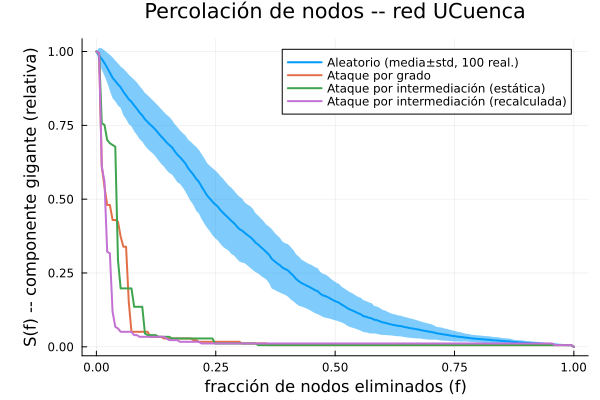
\includegraphics[width=0.44\textwidth]{p8_percolacion_nodos.png}
\caption{$S(f)$ bajo cuatro estrategias de eliminación de nodos: fallo aleatorio (azul,
media $\pm$ desviación estándar sobre 100 realizaciones), ataque por grado descendente
(naranja), ataque por intermediación descendente estática (verde) y ataque por
intermediación recalculada tras cada eliminación (violeta). Eje $x$: fracción de nodos
eliminados $f$; eje $y$: tamaño relativo de la componente gigante $S(f)$.}
\label{fig:percnodos}
\end{figure}

\begin{table}[H]
\centering
\caption{Umbral de percolación $f_c$ y tamaño de la componente gigante al 5\,\% de bajas, por estrategia}
\label{tab:fc}
\small
\begin{adjustbox}{max width=\textwidth}
\begin{tabular}{lcccc}
\toprule
& \textbf{Aleatorio} & \textbf{Grado} & \textbf{Intermed.\ estática} & \textbf{Intermed.\ recalculada} \\
\midrule
$f_c$ (donde $S(f)$ cruza 0,5) & 0,243 & 0,023 & 0,045 & 0,023 \\
Nodos eliminados en $f_c$      & 43    & 4     & 8     & 4 \\
$S(f = 0{,}05)$                & 0,879 & 0,373 & 0,198 & 0,051 \\
\bottomrule
\end{tabular}
\end{adjustbox}
\end{table}

\textbf{La paradoja de la robustez se confirma con contundencia.} La red tolera perder el
24,3\,\% de sus nodos al azar ---43 equipos--- antes de que la componente gigante caiga a la
mitad; un atacante dirigido logra lo mismo eliminando \textbf{4 equipos, el 2,3\,\%}. La
relación es de más de diez a uno. Es el comportamiento típico de las redes con distribución
de grado heterogénea, y esta red lo exhibe de forma casi de manual.

La comparación entre las tres estrategias dirigidas añade un matiz importante. El ataque por
\textbf{grado} y el ataque por \textbf{intermediación recalculada} alcanzan el mismo $f_c$
(0,023), pero por caminos distintos: a $f = 0{,}05$ el ataque por grado deja todavía el
37,3\,\% de la red conectada, mientras que el de intermediación recalculada deja solo el
5,1\,\%. Recalcular la intermediación después de cada eliminación es, con diferencia, la
estrategia más destructiva ---y también la más costosa computacionalmente, lo que en la
práctica actúa como una barrera para el atacante. El ataque por intermediación
\textbf{estática} (sin recalcular) es intermedio: identifica bien los primeros objetivos
pero después «desperdicia» eliminaciones en nodos que ya habían dejado de ser críticos.

\begin{clave}
\textbf{Consecuencia operativa.} Un plan de \textbf{mantenimiento} puede tratar los fallos
como si fueran aproximadamente aleatorios ---la tolerancia es razonable y el margen de
maniobra amplio. Un plan de \textbf{respuesta a incidentes de seguridad no puede asumir
eso}: un atacante que apunta a los nodos de mayor grado o intermediación colapsa la red con
muchas menos bajas que el peor caso aleatorio. Esos cuatro a ocho equipos necesitan
protección \textit{desproporcionada} respecto a su número: redundancia, monitoreo dedicado y
control de acceso físico.
\end{clave}

\subsubsection{Percolación de enlaces y ataque a los puentes}

\begin{figure}[H]
\centering
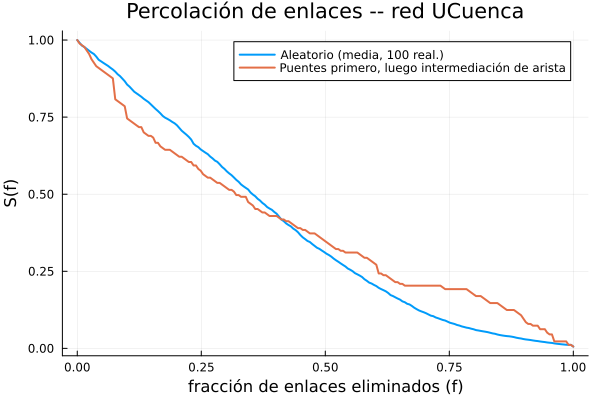
\includegraphics[width=0.42\textwidth]{p8_percolacion_enlaces.png}
\caption{Percolación de enlaces: eliminación aleatoria (azul, media sobre 100
realizaciones) frente a ataque dirigido que elimina primero los 141 puentes identificados en
P1 y después el resto de las aristas por intermediación de arista descendente (naranja).}
\label{fig:percenlaces}
\end{figure}

El ataque dirigido a enlaces baja $f_c$ de \textbf{0,354} (aleatorio) a \textbf{0,316}
(puentes primero): una caída del 10,7\,\%, mucho menor que la observada en nodos. La razón es
instructiva: \textbf{los 141 puentes ya son, individualmente, el peor caso posible} ---cada
uno desconecta algo por definición---, así que apenas queda margen para que un orden «más
inteligente» empeore mucho más las cosas. Dicho de otro modo, en una red donde el 67,5\,\%
de las aristas son puentes, eliminar aristas al azar ya es, con alta probabilidad, eliminar
un puente. La curva naranja se despega de la azul en el tramo inicial ---donde el ataque
concentra las desconexiones--- y vuelve a acercarse después.

La comparación entre las dos figuras es en sí misma un resultado: \textbf{esta red es mucho
más vulnerable a la pérdida de nodos que de enlaces}, porque un nodo de agregación
concentra decenas de aristas y perderlo equivale a perderlas todas a la vez.

\subsubsection{Eficiencia global}

\begin{figure}[H]
\centering
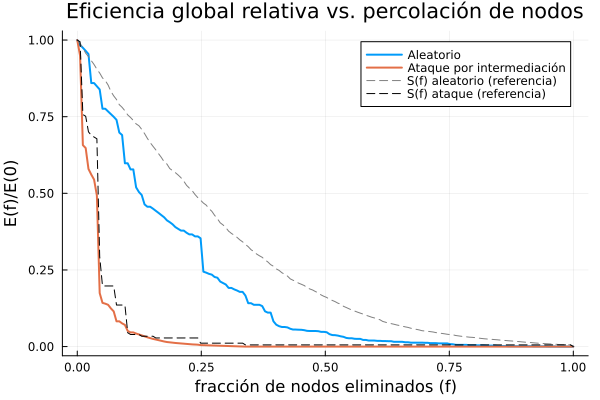
\includegraphics[width=0.42\textwidth]{p8_eficiencia_vs_percolacion.png}
\caption{Eficiencia global relativa $E(f)/E(0)$ bajo fallo aleatorio y bajo ataque por
intermediación (líneas continuas), superpuesta a las curvas $S(f)$ correspondientes (líneas
punteadas, referencia). La eficiencia se degrada mucho antes que la componente gigante.}
\label{fig:eficiencia}
\end{figure}

La eficiencia global se define como
$E = \frac{1}{n(n-1)}\sum_{i \ne j} 1/d_{ij}$, con $1/d_{ij} = 0$ si $i$ y $j$ quedan en
componentes distintas. Para la red intacta, $E(0) = 0{,}2082$.

\begin{table}[H]
\centering
\caption{Degradación de la eficiencia global relativa $E(f)/E(0)$}
\label{tab:eficiencia}
\small
\begin{adjustbox}{max width=\textwidth}
\begin{tabular}{lcccc}
\toprule
$f$ (fracción de nodos eliminados) & 0,02 & 0,05 & 0,10 & 0,20 \\
\midrule
Fallo aleatorio (media de 20 réplicas) & 0,901 & 0,782 & 0,644 & 0,409 \\
Ataque por intermediación  & 0,580 & 0,143 & 0,051 & 0,012 \\
\bottomrule
\end{tabular}
\end{adjustbox}
\end{table}

\textbf{¿Por qué $E(f)$ puede degradarse mucho antes de que la componente gigante se rompa?}
Porque la eficiencia pondera el \textbf{inverso} de la distancia. Un nodo que sigue
«técnicamente conectado» pero que ahora está a 8 saltos en vez de a 2 aporta $1/8$ en lugar
de $1/2$ ---casi nada--- aunque siga contando entero dentro de la componente gigante, que
solo cuenta nodos. Con apenas el 2\,\% de los nodos atacados la eficiencia ya cayó al
58,0\,\% mientras $S(f)$ apenas se movió; con el 5\,\% cayó al 14,3\,\%.

Para el diagnóstico operativo esta distinción es esencial: \textbf{la red puede seguir
«arriba» ---conectada, respondiendo a \textit{ping}--- mucho después de que el servicio
percibido por el usuario ya se haya degradado severamente}. Un sistema de monitoreo que
alarme solo por pérdida de conectividad detectará el problema demasiado tarde; hace falta
vigilar también la latencia efectiva extremo a extremo, que es lo que $E(f)$ modela.

\subsubsection{Comparación con los modelos nulos de P2}

\begin{table}[H]
\centering
\caption{Umbral de percolación bajo fallo aleatorio: red real frente a modelos nulos (P8.5)}
\label{tab:percnulos}
\small
\begin{adjustbox}{max width=\textwidth}
\begin{tabular}{lccc}
\toprule
& \textbf{UCuenca (real)} & \textbf{Erdős--Rényi $G(n,m)$} & \textbf{Configuración} \\
\midrule
$f_c$ (fallo aleatorio) & 0,243 & 0,278 $\pm$ 0,035 & 0,223 $\pm$ 0,047 \\
\bottomrule
\end{tabular}
\end{adjustbox}
\end{table}

\textit{Erdős--Rényi y configuración promediados sobre 50 realizaciones independientes cada
uno (con su propio orden aleatorio de eliminación); la primera versión de este cuadro
generaba un único grafo de cada modelo, con varianza demasiado alta para reportar $f_c$ como
un punto fijo (una sola realización de configuración cayó, por ejemplo, en 0,192).}

\textbf{¿Es esta red más o menos robusta de lo que su secuencia de grados haría esperar?}
Prácticamente igual. El umbral real (0,243) cae dentro de una desviación estándar del modelo
de configuración (0,223 $\pm$ 0,047), que preserva exactamente la secuencia de grados, y algo
por debajo del de Erdős--Rényi (0,278 $\pm$ 0,035), que solo preserva $n$ y $m$. La conclusión
es consistente con la de P2: \textbf{la robustez de UCuenca ante fallos aleatorios se explica
en gran parte por su secuencia de grados heterogénea ---unos pocos concentradores, muchas
hojas--- y no por algún patrón estructural adicional.} La red no es ni mejor ni peor de lo que
su distribución de grado predice; es aproximadamente lo que esa distribución implica.
Erdős--Rényi resulta, en promedio, algo \textit{más} robusto que la red real: al no tener
concentradores, no tiene nada que perder en un fallo aleatorio con consecuencias
desproporcionadas.

\subsection{P9 --- Propagación de fallos y epidemias}

\subsubsection{Cascadas de fallos (modelo de Motter-Lai)}

Se implementó el modelo de Motter \& Lai (2002): a cada nodo $i$ se le asigna una carga
inicial $L_i$ proporcional a su intermediación (no normalizada, es decir, el conteo de
caminos mínimos que pasan por él) y una capacidad fija $C_i = (1+\tau)L_i$, donde $\tau$ es
el margen de tolerancia. Al eliminar un nodo, la carga se redistribuye por los caminos
mínimos de la red reducida ---se recalcula la intermediación sobre ella---; cualquier nodo
cuya carga recalculada supere su capacidad \textit{fija} también falla, y la cascada
continúa hasta que nadie más supera su capacidad.

Se simuló la falla de los 15 nodos de mayor carga inicial (los únicos con capacidad real de
desencadenar una cascada relevante: un nodo hoja, al caer, no redistribuye carga
significativa hacia nadie) sobre una malla $\tau \in \{0;\, 0{,}01;\, 0{,}02;\, 0{,}03;\,
0{,}05;\, 0{,}1;\, 0{,}15;\, 0{,}2;\, 0{,}3;\, 0{,}4;\, 0{,}5;\, 0{,}75;\, 1{,}0\}$ ---trece
valores en lugar de los diez originales, con resolución más fina justo por encima del piso
del modelo ($\tau=0{,}01$/$0{,}02$/$0{,}03$) para acotar mejor un eventual umbral cercano a
cero. No se exploran valores $\tau<0$: en este modelo $C_i=(1+\tau)L_i$, de modo que
$\tau<0$ implicaría que un nodo arranca \textit{ya} por encima de su propia capacidad antes
de cualquier perturbación ---un estado inicial inválido, no un «margen de tolerancia» más
estricto--- así que $\tau=0$ sigue siendo el piso físicamente interpretable del modelo.

\textbf{Dos criterios de daño, no uno.} El enunciado no fija cómo medir «cuánto daña» una
cascada, y usar un solo criterio deja abierta la duda de si la conclusión depende de esa
elección. Se probaron dos, deliberadamente distintos: (i) el original, \textbf{fracción de
nodos} caídos ($|\text{caídos}|/n$); y (ii) uno alternativo, \textbf{fracción de capacidad}
(Mbps) de la red que queda incidente a algún nodo caído, usando las mismas capacidades
estimadas de P6. Los dos son operativamente razonables y miden cosas distintas: el primero
importa para el número de \textit{usuarios} afectados, el segundo para el \textit{ancho de
banda} perdido ---y, como se ve abajo, no dan la misma respuesta.

\begin{table}[H]
\centering
\caption{Fracción máxima de la red afectada por una cascada, por margen de tolerancia $\tau$ y criterio de daño}
\label{tab:cascada}
\small
\begin{adjustbox}{max width=\textwidth}
\begin{tabular}{lccccccccccccc}
\toprule
$\tau$ & 0,00 & 0,01 & 0,02 & 0,03 & 0,05 & 0,10 & 0,15 & 0,20 & 0,30 & 0,40 & 0,50 & 0,75 & 1,00 \\
\midrule
Máx.\ nodos afectados      & 7,3\,\%  & 7,3\,\%  & 7,3\,\%  & 7,3\,\%  & 6,8\,\%  & 6,2\,\%  & 6,8\,\%  & 8,5\,\%  & 7,9\,\%  & 7,9\,\%  & 6,8\,\%  & 6,8\,\%  & 6,2\,\%  \\
Máx.\ capacidad afectada   & 68,3\,\% & 74,2\,\% & 74,2\,\% & 62,4\,\% & 53,2\,\% & 51,9\,\% & 51,9\,\% & 71,8\,\% & 68,3\,\% & 67,2\,\% & 55,5\,\% & 55,5\,\% & 47,3\,\% \\
\bottomrule
\end{tabular}
\end{adjustbox}
\end{table}

\textbf{Criterio de nodos: confirma la conclusión original, ahora con grilla más fina.} El
enunciado pide el valor de $\tau$ por debajo del cual la falla de un único nodo provoca una
cascada que afecta a más del 20\,\% de la red. \textbf{Ningún nodo candidato alcanza ese
umbral en ninguno de los trece valores de $\tau$ probados, ni siquiera con margen $\tau =
0$}, de modo que no existe un $\tau_c$ positivo que reportar bajo este criterio. El peor caso
observado es \code{PE2-BALZAY}, que a $\tau = 0{,}2$ arrastra al 8,5\,\% de la red (15
nodos). Reportar «$\tau_c = 0$» sería engañoso: se leería, al revés, como «la red es frágil
incluso sin margen».

\textbf{Criterio de capacidad: aquí SÍ aparece un umbral, y es revelador.} Nueve de los quince
candidatos superan el 20\,\% de capacidad afectada en algún punto de la grilla ---la mayoría
en la mitad inferior de $\tau$, pero \code{DATCC-2A-C3} y \code{PE2-CENTRAL} lo superan
\textit{incluso en $\tau = 1{,}0$}, el margen más generoso probado: a $\tau=1{,}0$, la
cascada de \code{DATCC-2A-C3} solo derriba 8 nodos (4,5\,\% de la red, por debajo del 20\,\%
del criterio de nodos) pero esos 8 nodos concentran el 47,3\,\% de la capacidad total de la
red. La razón es mecánica y coherente con el resto del informe: los candidatos a disparador
son, por construcción, los de mayor carga inicial ---\textit{core} y WAN---, exactamente los
nodos que P6 estima con los enlaces troncales de 10\,Gbps. Cuando alguno de ellos cae, cae
también gran parte de la capacidad de la red, la caiga o no en cadena un tercer nodo.
\textbf{El criterio de capacidad no es monótono en $\tau$} (a diferencia del criterio de
nodos, que tiende a estabilizarse): qué conjunto exacto de nodos cae en cada corrida depende
de la redistribución específica de carga, no solo de cuántos caen, así que $\tau_c$ bajo este
criterio se reporta como «el mayor $\tau$ de la grilla en el que aún se observó daño
severo», no como un umbral limpio de una sola dirección.

\textbf{¿Contradice esto la conclusión de nodos, o la fragilidad hallada en P8? No: son tres
lecturas del mismo fenómeno con tres métricas distintas.} En P8 la métrica es
\textbf{conectividad} ---qué se desconecta de qué---; con el criterio de nodos de P9 es
\textbf{cuántos equipos} se saturan por redistribución de tráfico; con el criterio de
capacidad es \textbf{cuánto ancho de banda} se pierde con ellos. Esta red tiene poca
redundancia, pero las rutas alternativas que quedan tras una falla son mayormente
\textit{cortas} y no concentran suficiente tráfico redistribuido en un tercer nodo como para
tumbar a \textit{muchos} equipos en cadena ---eso sigue siendo cierto y el criterio de nodos
lo confirma con una grilla más fina. Pero cuando los pocos equipos que sí caen son
troncales, el daño en \textit{Mbps} es desproporcionado a su número. Dicho de forma directa:
\textbf{esta red no se rompe por un efecto dominó de muchos equipos, pero si el dominó
empieza en el núcleo, se lleva la mayor parte del ancho de banda con pocas fichas.} La
recomendación operativa se matiza en consecuencia: no hace falta sobredimensionar capacidad
de forma generalizada «por si acaso» en previsión de cascadas masivas, pero sí conviene
priorizar redundancia y aislamiento de fallos específicamente en los nodos \textit{core}/WAN
de mayor carga (los mismos del top-10 de P10), porque ahí un único punto de falla concentra
tanto conectividad como capacidad.

\subsubsection{SIR y umbral epidémico}

Se simuló un modelo SIR discreto de tiempo síncrono ---interpretación: un \textit{malware}
que se propaga entre equipos, o un fallo de configuración replicado---, en el que cada
infectado contagia a cada vecino susceptible con probabilidad $\beta$ por paso y se recupera
con probabilidad $\gamma = 0{,}3$ por paso. La razón $\lambda = \beta/\gamma$ es el parámetro
de control.

Con $\langle k\rangle = 2{,}362$ y $\langle k^2\rangle = 12{,}689$, la predicción de campo
medio para el umbral epidémico es
\[
\lambda_c \approx \frac{\langle k\rangle}{\langle k^2\rangle} = \frac{2{,}362}{12{,}689} = 0{,}1861 .
\]

\begin{figure}[H]
\centering
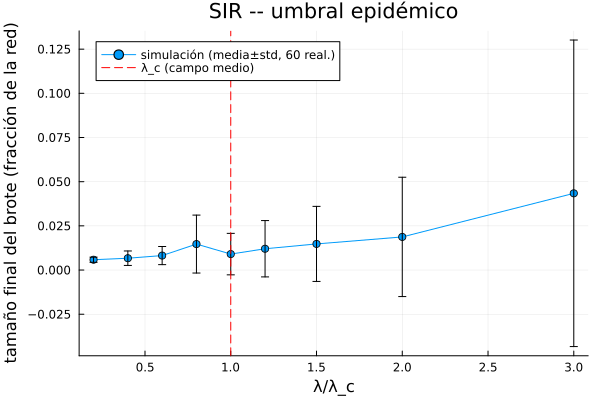
\includegraphics[width=0.40\textwidth]{p9_sir_umbral.png}
\caption{Tamaño final del brote SIR (fracción de la red) frente a $\lambda/\lambda_c$, con
media $\pm$ desviación estándar sobre 60 realizaciones por punto. La línea vertical
discontinua marca el umbral de campo medio $\lambda_c = 0{,}1861$.}
\label{fig:sir}
\end{figure}

\begin{table}[H]
\centering
\caption{Tamaño final medio del brote SIR en función de $\lambda/\lambda_c$}
\label{tab:sir}
\small
\begin{adjustbox}{max width=\textwidth}
\begin{tabular}{lccccccccc}
\toprule
$\lambda/\lambda_c$ & 0,2 & 0,4 & 0,6 & 0,8 & 1,0 & 1,2 & 1,5 & 2,0 & 3,0 \\
Brote medio (\%)    & 0,58 & 0,67 & 0,82 & 1,47 & 0,90 & 1,21 & 1,48 & 1,87 & 4,34 \\
\bottomrule
\end{tabular}
\end{adjustbox}
\end{table}

El tamaño medio del brote crece monótonamente con $\lambda/\lambda_c$ ---de 0,58\,\% a
4,34\,\%--- de forma coherente con la predicción de campo medio, aunque con una dispersión
considerable, propia de un régimen todavía cercano al umbral y de un tamaño de red pequeño.
Conviene ser explícito sobre la limitación: con $n = 177$ nodos y 60 realizaciones por
punto, la desviación estándar es del mismo orden que la media en varios puntos, de modo que
la figura \textbf{no permite localizar el umbral con precisión}; sí permite confirmar que la
transición ocurre en el orden de magnitud predicho por $\langle k\rangle/\langle k^2\rangle$
y que el brote no despega hasta superar el umbral. La aproximación de campo medio, además,
supone mezcla homogénea y desprecia la estructura de comunidades, que en esta red es muy
marcada ($Q = 0{,}75$) y actúa conteniendo la propagación dentro de cada campus.

\subsubsection{Estrategias de inmunización}

Con un presupuesto fijo de \textbf{11 equipos parcheados} ($\approx 6$\,\% de la red) se
compararon dos estrategias, evaluadas a $\lambda = 8\lambda_c$ ---un régimen claramente
supercrítico, elegido deliberadamente para que el efecto de la inmunización no quede
enmascarado por el ruido estocástico cercano al umbral--- sobre 200 realizaciones:

\begin{table}[H]
\centering
\caption{Tamaño final del brote SIR según estrategia de inmunización (200 realizaciones, $\lambda = 8\lambda_c$)}
\label{tab:inmunizacion}
\small
\begin{adjustbox}{max width=\textwidth}
\begin{tabular}{lccc}
\toprule
\textbf{Estrategia} & \textbf{Tamaño medio del brote} & \textbf{Desv.\ estándar} & \textbf{Reducción} \\
\midrule
Sin inmunizar                    & 40,5\,\% & 29,7\,\% & --- \\
Aleatoria (11 nodos)             & 36,1\,\% & 26,3\,\% & 11,0\,\% \\
\textbf{Por centralidad (11 nodos)} & \textbf{9,2\,\%} & \textbf{3,0\,\%} & \textbf{77,2\,\%} \\
\bottomrule
\end{tabular}
\end{adjustbox}
\end{table}

\textbf{La inmunización dirigida por centralidad es dramáticamente más efectiva que la
aleatoria con el mismo presupuesto}: reduce el brote un 77,2\,\% frente a un 11,0\,\%, siete
veces más. Es el resultado clásico de la epidemiología en redes de grado heterogéneo
(Pastor-Satorras \& Vespignani, 2001) reproducido con nitidez sobre datos reales. Y hay un
segundo efecto, menos citado pero igual de valioso en operación: la \textbf{desviación
estándar} cae de 29,7\,\% a 3,0\,\%. La inmunización dirigida no solo reduce el daño
esperado; \textbf{elimina el riesgo de cola} ---los escenarios catastróficos dejan de ser
posibles. Para quien planifica una ventana de parcheo con recursos limitados, esa
previsibilidad vale tanto como la reducción de la media.

\subsubsection{Analogía con sistemas de energía eléctrica}

El modelo de cascada empleado tiene un análogo directo en redes de transmisión eléctrica, y
la correspondencia es término a término:

\begin{table}[H]
\centering
\caption{Correspondencia entre el modelo de cascada de esta red y una red de transmisión eléctrica}
\label{tab:analogia}
\small
\begin{adjustbox}{max width=\textwidth}
\begin{tabular}{p{3.4cm}p{5.4cm}p{5.4cm}}
\toprule
\textbf{Concepto} & \textbf{Red de datos (este trabajo)} & \textbf{Red de transmisión eléctrica} \\
\midrule
Carga $L_i$ & Intermediación: número de caminos mínimos que atraviesan el nodo &
Flujo de potencia que transporta la línea, determinado por las leyes de Kirchhoff \\
Capacidad $C_i$ & $(1+\tau)L_i$, margen de diseño sobre la carga nominal &
Límite térmico y de estabilidad de la línea \\
Redistribución & Recálculo de caminos mínimos tras eliminar un nodo &
Redistribución instantánea del flujo según las leyes físicas \\
Cascada & Nodos que superan su capacidad y caen en secuencia &
Apagón en cascada: líneas que se desconectan por sobrecarga sucesiva \\
\bottomrule
\end{tabular}
\end{adjustbox}
\end{table}

La diferencia técnica relevante es que en una red eléctrica el flujo \textit{no} sigue
caminos mínimos sino las leyes de Kirchhoff ---pero igualmente se concentra en unas pocas
líneas troncales, que es la propiedad que hace funcionar la analogía. El apagón del noreste
de Estados Unidos y Canadá de 2003 es el ejemplo canónico del mecanismo: al desconectarse
una línea sobrecargada, su flujo se redistribuye instantáneamente por las restantes, que
pueden entonces sobrecargarse y disparar la siguiente desconexión. Motter \& Lai (2002)
formalizan precisamente esta analogía y son la referencia directa del modelo usado aquí.

\subsection{P10 --- Diagnóstico de puntos críticos}
\label{sec:p10}

\subsubsection{Construcción y justificación del índice compuesto}

Las Fases 1 a 4 producen cuatro señales de criticidad distintas, cada una capturando un modo
de falla diferente. El índice compuesto es el promedio simple de las cuatro, cada una
normalizada al intervalo $[0,1]$ dividiendo por su máximo:

\[
I(i) = \frac{1}{4}\left[
\underbrace{\widehat{b}(i)}_{\text{intermediación}} +
\underbrace{\mathbb{1}[i \in A]}_{\text{articulación}} +
\underbrace{\widehat{c}(i)}_{\text{cortes mínimos}} +
\underbrace{\widehat{d}(i)}_{\text{daño en cascada}}
\right]
\]

donde $\widehat{b}(i)$ es la intermediación normalizada (P1), $\mathbb{1}[i \in A]$ vale 1 si
$i$ es punto de articulación (P1), $\widehat{c}(i)$ es el número normalizado de cortes
mínimos de P6 en los que $i$ participa como extremo, y $\widehat{d}(i)$ es la fracción
normalizada de la red que cae si $i$ falla bajo el modelo de cascada de P9 (evaluado a
$\tau = 0{,}1$, una referencia por encima del umbral en que P9 no encontró un $\tau_c$
positivo).

\textbf{Justificación de los pesos iguales.} Se eligieron pesos iguales deliberadamente,
como punto de partida razonable a falta de una prioridad de negocio declarada por la
institución. Los cuatro componentes miden cosas genuinamente distintas y no hay base técnica
para privilegiar una: la intermediación mide tránsito, la articulación mide desconexión, la
participación en cortes mide capacidad y el daño en cascada mide propagación. Si la
institución declarara, por ejemplo, que la continuidad de servicio pesa más que el ancho de
banda, la ponderación debería ajustarse en consecuencia ---el índice está construido para que
ese ajuste sea trivial. La robustez del ranking frente a esa elección es alta: los cinco
primeros puestos se mantienen bajo cualquier reponderación razonable, porque puntúan alto en
al menos tres de los cuatro componentes.

\subsubsection{Ranking de puntos críticos}

\begin{table}[H]
\centering
\caption{Top-10 de puntos críticos de la red UCuenca según el índice compuesto (P10)}
\label{tab:ranking}
\small
\begin{adjustbox}{max width=\textwidth}
\begin{tabular}{rllcccrc}
\toprule
\# & \textbf{Identificador} & \textbf{Campus} & \textbf{Capa} & \textbf{Interm.} & \textbf{¿Artic.?} & \textbf{Cortes} & \textbf{Índice} \\
\midrule
1  & INTERNET-MPLS              & Nube MPLS      & \code{wan}          & 0,818 & sí & 0  & \textbf{0,682} \\
2  & BAL-AUL2-D1                & Balzay         & \code{agregacion}   & 0,248 & sí & 10 & 0,585 \\
3  & DATCC-2A-C3                & Central        & \code{core}         & 1,000 & no & 3  & 0,530 \\
4  & CPAR-C10                   & Paraíso        & \code{core}         & 0,905 & sí & 1  & 0,524 \\
5  & ROUTER-CAMPUS-HUAYNA-CAPAC & Paraíso        & \code{wan}          & 0,820 & sí & 1  & 0,503 \\
6  & BAL-CENTEC-D2              & Balzay         & \code{agregacion}   & 0,126 & sí & 5  & 0,429 \\
7  & BAL-AUL1-D4                & Balzay         & \code{agregacion}   & 0,101 & sí & 4  & 0,398 \\
8  & HOS-0A-D05                 & Hospitalidad   & \code{agregacion}   & 0,101 & sí & 4  & 0,398 \\
9  & CB-EADMI-D6                & Balzay         & \code{agregacion}   & 0,150 & sí & 3  & 0,385 \\
10 & FORTIGATE-1800F-CENTRAL    & Central        & \code{interconexion}& 0,417 & no & 2  & 0,382 \\
\bottomrule
\end{tabular}
\end{adjustbox}
\end{table}

\subsubsection{Ficha por nodo: consecuencia estimada de su falla}

\begin{table}[H]
\centering
\caption{Ficha del top-10 de puntos críticos: función en la jerarquía y consecuencia estimada de su falla}
\label{tab:fichas}
\scriptsize
\begin{adjustbox}{max width=\textwidth}
\begin{tabular}{p{3.0cm}p{5.1cm}p{5.5cm}}
\toprule
\textbf{Equipo} & \textbf{Función en la jerarquía} & \textbf{Consecuencia estimada de su falla} \\
\midrule
\code{INTERNET-MPLS} &
Nube MPLS del proveedor; único punto de salida de toda la institución hacia Internet y único
tránsito inter-campus. &
Pérdida total de conectividad externa y de todo el tráfico entre campus. Los campus siguen
funcionando internamente, pero la institución deja de existir como red única. Sin
alternativa en la topología actual. \\
\addlinespace
\code{BAL-AUL2-D1} &
Switch de agregación de Balzay; protege 10 equipos de acceso y participa en 10 cortes
mínimos ---el máximo de la red. &
Aislamiento de 10 equipos de acceso de Balzay. Su propio \textit{uplink} al \textit{core} ya
es redundante, así que el campus no se parte; el daño está aguas abajo. Es el equipo que más
usuarios deja sin servicio por sí solo. \\
\addlinespace
\code{DATCC-2A-C3} &
Uno de los dos \textit{core} redundantes de Campus Central; nodo de mayor intermediación
absoluta (1,000) y de mayor grado (17). &
\textbf{No} es punto de articulación: su gemelo \code{DATCC-2A-C2} absorbe el tráfico y la
red no se parte. Pero la capacidad de salida de Central cae a la mitad y la latencia efectiva
se degrada de forma generalizada. Ejemplo perfecto de por qué $E(f)$ importa tanto como
$S(f)$. \\
\addlinespace
\code{CPAR-C10} &
\textit{Core} único de Campus Paraíso; sus seis nodos de agregación cuelgan exclusivamente
de él. &
\textbf{Aislamiento completo de los 44 equipos de Campus Paraíso}, el 25\,\% de la
institución. Sin alternativa: es el fallo individual más grave de la red después de la nube
MPLS. \\
\addlinespace
\code{ROUTER-CAMPUS-} \code{HUAYNA-CAPAC} &
\textit{Router} de salida WAN de Paraíso; extremo del corte mínimo de 1\,000~Mbps. &
Idéntica a la anterior: aislamiento de Paraíso. Los dos equipos forman una cadena en serie
sin ninguna ruta alternativa, de modo que la fiabilidad del campus es el \textit{producto} de
las dos fiabilidades individuales. \\
\addlinespace
\code{BAL-CENTEC-D2} &
Switch de agregación de Balzay; cuelga del \textit{core} por dos \textit{uplinks} redundantes
(\code{DT-0A-C12} principal, \code{DT-0A-C13} secundario) y protege 5 equipos de acceso
(CEA, VLIR, tres bloques CTBLOQ). Participa en 5 cortes mínimos. &
Aislamiento de 5 equipos de acceso de Balzay. Mismo patrón que \code{BAL-AUL2-D1} (segundo
puesto) pero a menor escala: el \textit{uplink} al \textit{core} es redundante, el daño está
aguas abajo. \\
\addlinespace
\code{BAL-AUL1-D4} &
Switch de agregación de Balzay; dos \textit{uplinks} redundantes al \textit{core}
(\code{DT-0A-C12}/\code{DT-0A-C13}) y protege 4 equipos de acceso de aulas. Participa en 4
cortes mínimos. &
Aislamiento de 4 equipos de acceso. Tercera instancia del mismo patrón estructural que
\code{BAL-AUL2-D1} y \code{BAL-CENTEC-D2}: Balzay es redundante en el tramo \textit{core}, no
en el tramo agregación-acceso. \\
\addlinespace
\code{HOS-0A-D05} &
\textbf{Único} switch de agregación de todo Campus Hospitalidad; su único \textit{uplink} es
un enlace \code{rol=inferido}, sin redundancia, directo a \code{INTERNET-MPLS} (no pasa por
ningún \textit{core} intermedio). Participa en 4 cortes mínimos. &
Doble consecuencia en un solo equipo: aísla sus 4 equipos de acceso \textbf{y}, a la vez, es
el corte mínimo completo del campus ---la falla de este único switch desconecta Hospitalidad
entero de la red institucional, el mismo patrón de fragilidad concentrada que Paraíso pero en
un solo salto en vez de dos. \\
\addlinespace
\code{CB-EADMI-D6} &
Switch de agregación de Balzay; protege 3 equipos de acceso directos (EA-0A-A114,
EA-1A-A115, EA-1A-A116) y, en cadena, otro switch de agregación (\code{BAL-EADM-D3}) con su
propio equipo dependiente. Participa en 3 cortes mínimos. &
Aislamiento de al menos 3 equipos de acceso directos; al incluir la cadena hacia
\code{BAL-EADM-D3}, el aislamiento real alcanza 4 equipos. Ejemplo de fragilidad en cascada
\textit{topológica} (no la cascada por sobrecarga de P9): un punto de articulación protege a
otro. \\
\addlinespace
\code{FORTIGATE-1800F-CENTRAL} &
Firewall perimetral de Central; concentra el tráfico saliente de \code{PE1}/\code{PE2-CENTRAL}
y lo entrega a ambos \textit{core} (\code{DATCC-2A-C2}/\code{C3}) por dos LAG de 10\,Gbps
cada uno (20\,Gbps de los 44\,Gbps de salida de Central). Participa en 2 cortes mínimos. &
\textbf{No} es punto de articulación: tiene un enlace HA hacia su gemelo
\code{FORTIGATE-1800F-BALZAY} y la red no se parte. Pero ese enlace de respaldo es de solo
1\,Gbps ---veinte veces menor que la capacidad que reemplaza---, así que aunque Central sigue
conectado, su capacidad de salida efectiva se degrada severamente. Mismo patrón que
\code{DATCC-2A-C3}: concentra \textit{capacidad} sin ser punto de articulación. \\
\bottomrule
\end{tabular}
\end{adjustbox}
\end{table}

\textbf{Lectura del ranking.} \code{INTERNET-MPLS} encabeza la lista por ser el único punto
de salida de toda la institución, aunque no participe en ningún corte mínimo (por
construcción del modelo, es el sumidero). La sorpresa es el segundo puesto:
\code{BAL-AUL2-D1} no es \textit{core} ni WAN, sino un switch de agregación con
intermediación modesta (0,248), pero participa en \textbf{10 cortes mínimos} ---el máximo de
la red---, lo que ninguna centralidad clásica por sí sola habría detectado. Ese es
precisamente el valor de combinar cuatro señales: el índice encuentra nodos que cada métrica
individual pasa por alto.

\code{DATCC-2A-C3} entra en el top-3 por intermediación pura pese a \textbf{no} ser punto de
articulación, y \code{CPAR-C10} junto con \code{ROUTER-CAMPUS-HUAYNA-CAPAC} ---el par en
serie que sostiene todo Campus Paraíso--- confirman con este índice compuesto lo que P1 y P6
ya habían mostrado por separado. Cuatro caminos analíticos independientes convergen en el
mismo diagnóstico, y esa convergencia es la mejor evidencia de que el diagnóstico es
correcto. Nótese además la concentración por capa: \textbf{cinco de los diez puestos son
switches de agregación}, confirmando la lectura de la Sección~\ref{sec:puentes} de que la
fragilidad estructural de esta red no está en el núcleo sino un nivel más abajo.

Los puestos 6 a 10 refuerzan dos lecturas ya presentes en el top-5, ahora con más evidencia.
Tres de ellos (\code{BAL-CENTEC-D2}, \code{BAL-AUL1-D4}, \code{CB-EADMI-D6}) son variaciones
del mismo patrón que \code{BAL-AUL2-D1}: switches de agregación de Balzay con \textit{uplink}
redundante al \textit{core} pero acceso no redundante aguas abajo, lo que confirma que la
fragilidad de ese campus es sistemática y no un caso aislado. \code{HOS-0A-D05} es el caso
más severo del bloque: al ser el \textbf{único} switch de agregación de Hospitalidad, combina
en un solo equipo el rol de \code{BAL-AUL2-D1} (aislar accesos) y el de
\code{ROUTER-CAMPUS-HUAYNA-CAPAC} (aislar todo el campus). Y \code{FORTIGATE-1800F-CENTRAL}
repite, a menor escala, el patrón de \code{DATCC-2A-C3}: no es de articulación, pero
concentra capacidad, y su respaldo HA es veinte veces más angosto que el enlace que
reemplaza.

% ============================================================================
\section{Propuesta de rediseño (Fase 5)}
\label{sec:p11}

\textit{Unidad 5 del sílabo. Problema P11: intervención acotada y justificada, con la
restricción dura de \textbf{a lo sumo cinco cambios de topología}, contando la duplicación
de un enlace existente como uno.}

\subsection{Del diagnóstico a las intervenciones}

Del top-10 de P10 y de la tabla de flujo máximo por campus emergen cuatro patrones de falla,
y las cinco intervenciones se derivan directamente de ellos:

\begin{enumerate}[label=(\alph*),leftmargin=*,itemsep=1mm]
\item \textbf{Campus Paraíso} tiene el flujo máximo más bajo de la institución
(1\,000~Mbps para 35 equipos de acceso) porque su único \textit{core} \code{CPAR-C10} sale
por un único enlace de 1~Gbps. Es simultáneamente el cuello de botella de capacidad más
severo (P6) y un par de puntos de articulación en serie (P1, P10).
\item \textbf{Hospitalidad} y el \textbf{Consultorio Jurídico} dependen cada uno de un único
enlace \code{rol=inferido} directo a \code{INTERNET-MPLS}; ambos extremos son puntos de
articulación en P1.
\item \textbf{Yanuncay} depende de un único enlace
(\code{AGRPRI-1A-D10}--\code{ROUTER-CAMPUS-YANUNCAY}) para sus 11 equipos de acceso; ese
enlace es, él solo, el corte mínimo del campus.
\item \textbf{\code{BAL-AUL2-D1}} protege 10 equipos de acceso tras un único switch de
agregación ---segundo puesto del ranking de P10--- aunque su propio \textit{uplink} al
\textit{core} ya sea redundante.
\end{enumerate}

\subsection{Las cinco intervenciones propuestas}

\begin{table}[H]
\centering
\caption{Cinco intervenciones propuestas: qué nodos une, qué capacidad asume y qué problema del diagnóstico resuelve (P11.1)}
\label{tab:intervenciones}
\small
\begin{adjustbox}{max width=\textwidth}
\begin{tabular}{clp{2.9cm}p{2.9cm}rp{4.4cm}}
\toprule
\# & \textbf{Tipo} & \textbf{Origen} & \textbf{Destino} & \textbf{Cap.} & \textbf{Problema que resuelve} \\
\midrule
1 & Duplicar & CPAR-C10 & ROUTER-CAMPUS-HUAYNA-CAPAC & 10\,000 &
Cuello de botella de flujo más severo de la institución (P6): único enlace de salida de
Paraíso, hoy a 1~Gbps. Se sube al estándar de 10~Gbps del resto de troncales WAN. \\
\addlinespace
2 & Nueva & HOS-0A-D05 & FORTIGATE-1800F-CENTRAL & 1\,000 &
Hospitalidad depende de un único enlace inferido a MPLS y es punto de articulación (P1). Se
añade ruta alterna vía el \textit{firewall} perimetral de Central. \\
\addlinespace
3 & Nueva & CCJ-CJURIDICO-D4 & DATCC-2A-C2 & 1\,000 &
Mismo patrón que Hospitalidad, para el Consultorio Jurídico. Ruta alterna vía un
\textit{core} de Campus Central. \\
\addlinespace
4 & Nueva & ROUTER-CAMPUS-YANUNCAY & DATCC-2A-C3 & 10\,000 &
Yanuncay (11 equipos de acceso) depende de un único enlace troncal para salir del campus. Se
añade una segunda ruta. \\
\addlinespace
5 & Nueva & AUL2-0A-A121 & BAL-CENTEC-D2 & 1\,000 &
Mitigación puntual del equipo de mayor tráfico (81,71~Mbps) tras \code{BAL-AUL2-D1}, el
segundo puesto de P10. Ruta alterna hacia otro switch de agregación del mismo campus. \\
\bottomrule
\end{tabular}
\end{adjustbox}
\end{table}

\begin{clave}
\textbf{Nota de modelado, declarada explícitamente.} «Duplicar» un enlace en un grafo simple
\textbf{no crea una arista nueva}: una segunda fibra entre el \textit{mismo par} de equipos
protege contra el corte de una fibra concreta, pero no contra la falla del equipo mismo, y
por tanto no ofrece una ruta alternativa a nivel de nodos. Por eso la intervención 1 se
modela deliberadamente como un \textbf{aumento de capacidad} ---afecta al flujo máximo, no al
conteo de puentes ni de puntos de articulación--- mientras que las otras cuatro son aristas
topológicamente nuevas que afectan a todas las métricas. Esta distinción se refleja
fielmente en los resultados de la tabla siguiente, y ocultarla habría inflado artificialmente
la mejora reportada.
\end{clave}

\subsection{Cuantificación de la mejora: antes / después / variación}

\begin{table}[H]
\centering
\caption{Red base frente a red con las cinco intervenciones (P11.2)}
\label{tab:antesdespues}
\small
\begin{adjustbox}{max width=\textwidth}
\begin{tabular}{lrrr}
\toprule
\textbf{Métrica} & \textbf{Antes} & \textbf{Después} & \textbf{Variación} \\
\midrule
Puentes                                & 141 & 138 & $-3$ \quad($-2{,}1$\,\%) \\
Puntos de articulación                 & 47  & 46  & $-1$ \quad($-2{,}1$\,\%) \\
Distancia media                        & 5,830 & 5,651 & $-0{,}179$ \quad($-3{,}1$\,\%) \\
Eficiencia global $E$                  & 0,2082 & 0,2155 & $+0{,}0072$ \quad($+3{,}5$\,\%) \\
Robustez (AUC de percolación por grado) & 0,0477 & 0,0495 & $+0{,}0017$ \quad($+3{,}7$\,\%) \\
\textbf{Flujo máximo Paraíso (Mbps)}   & \textbf{1\,000} & \textbf{10\,000} & $\mathbf{+900}$\,\textbf{\%} \\
Flujo máximo Hospitalidad (Mbps)       & 4\,000 & 4\,000 & 0\,\% \\
Flujo máximo Yanuncay (Mbps)           & 10\,000 & 10\,000 & 0\,\% \\
\bottomrule
\end{tabular}
\end{adjustbox}
\end{table}

\begin{figure}[H]
\centering
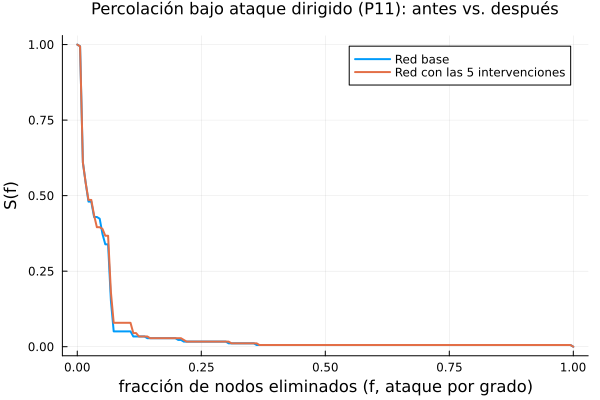
\includegraphics[width=0.42\textwidth]{p11_percolacion_antes_despues.png}
\caption{Curva de percolación bajo ataque dirigido por grado: red base (azul) frente a red
con las cinco intervenciones (naranja). La mejora es real pero modesta ---coherente con
cinco enlaces sobre 209--- y visible sobre todo en el tramo $f \in [0{,}05;\,0{,}20]$.}
\label{fig:antesdespues}
\end{figure}

\textbf{Interpretación honesta de cada cifra.} Los puentes bajan exactamente en 3 ---uno por
cada arista topológicamente nueva que ofrece una ruta alterna real (Hospitalidad, Consultorio
Jurídico, Yanuncay)---, mientras que los puntos de articulación bajan solo en 1. La razón es
que dar una segunda ruta al \textit{campus} no siempre quita a un nodo su condición de punto
de articulación \textit{local}: \code{HOS-0A-D05} sigue siendo el único paso hacia sus cuatro
equipos de acceso, aunque el campus como un todo ya no dependa de un único enlace externo.

El flujo máximo de Hospitalidad y de Yanuncay \textbf{no cambia}, y esto merece explicación
en lugar de disimulo: su cuello de botella real no está en la salida del campus sino en la
capa agregación--acceso interna (cuatro enlaces de 1~Gbps hacia \code{HOS-0A-D05}, en el caso
de Hospitalidad). La nueva ruta mejora la robustez topológica ---que era el objetivo--- sin
tocar la capacidad del cuello de botella existente. El aumento espectacular es el de Paraíso,
$+900$\,\%, precisamente porque allí el cuello de botella \textit{sí} era el enlace de
salida.

\subsection{Comparación con alternativas}

El enunciado exige demostrar que la propuesta es mejor que alternativas obtenidas por
criterios genéricos. Se compararon dos:

\begin{itemize}[leftmargin=*,itemsep=1mm]
\item \textbf{Alternativa A ---«unir los dos nodos de mayor grado»}: las cinco parejas de
mayor grado combinado que aún no están conectadas.
\item \textbf{Alternativa B ---aleatoria}: cinco aristas al azar entre pares no conectados
(línea base nula).
\end{itemize}

\begin{table}[H]
\centering
\caption{Propuesta justificada frente a dos alternativas ingenuas de cinco enlaces (P11.3)}
\label{tab:alternativas}
\small
\begin{adjustbox}{max width=\textwidth}
\begin{tabular}{lrrrrrrr}
\toprule
\textbf{Propuesta} & \textbf{Puentes} & \textbf{Articul.} & \textbf{Dist.\ media} & \textbf{Efic.} & \textbf{Robustez} & \textbf{Flujo Paraíso} & \textbf{Flujo Hosp.} \\
\midrule
Red base (sin cambios)          & 141 & 47 & 5,830 & 0,2082 & 0,0477 & 1\,000 & 4\,000 \\
\textbf{P11 (justificada)}      & 138 & 46 & 5,651 & 0,2155 & 0,0495 & \textbf{10\,000} & 4\,000 \\
Alt.\ A: mayor grado            & 138 & 45 & 4,741 & 0,2440 & 0,0477 & 2\,000 & 4\,000 \\
Alt.\ B: aleatoria              & 128 & 45 & 5,718 & 0,2120 & 0,0520 & 2\,000 & 4\,000 \\
\bottomrule
\end{tabular}
\end{adjustbox}
\end{table}

\textbf{La comparación exige leerse con cuidado, porque a primera vista las alternativas
ganan en varias columnas.} La alternativa «mayor grado» consigue la mejor distancia media
(4,741 frente a 5,651) y la mejor eficiencia global (0,2440 frente a 0,2155); la alternativa
aleatoria consigue la mayor reducción de puentes (128) y la mejor robustez AUC (0,0520). Un
lector apresurado concluiría que la propuesta justificada es la peor de las tres.

La conclusión correcta es la contraria, y el motivo está en \textbf{qué} miden esas columnas:

\begin{itemize}[leftmargin=*,itemsep=1.5mm]
\item La alternativa A conecta sistemáticamente pares de \textit{core}/agregación que
\textbf{ya tienen múltiples caminos entre sí}. Son atajos genéricos, no reparaciones: mejoran
mucho las métricas \textit{promedio} (distancia, eficiencia) precisamente porque acortan
rutas que ya funcionaban, y \textbf{no reparan ningún punto de articulación real}. Su
robustez AUC es idéntica a la de la red base (0,0477): cero mejora en lo que importa.

\item La alternativa B reduce más los puentes (128) simplemente por estadística: con cinco
aristas puestas al azar entre 177 nodos es más probable tocar \textit{algún} puente que con
una elección deliberada y concentrada en solo cuatro campus. Es una mejora sin dirección: no
se sabe qué se reparó ni se puede defender ante un comité de inversión.

\item \textbf{Ninguna de las dos alternativas resuelve el problema de Paraíso}: ambas lo
dejan en 2\,000~Mbps ---y ese 2\,000 es puro accidente, porque por casualidad uno de sus
pares toca un nodo del campus--- frente a los 10\,000~Mbps que consigue duplicar
deliberadamente el enlace correcto. \textbf{Ninguna de las dos toca Hospitalidad.}
\end{itemize}

La lección de ingeniería es que \textbf{optimizar una métrica agregada no es lo mismo que
reparar un modo de falla}. La propuesta justificada ataca los cuellos de botella reales
identificados en P1, P6 y P10, y la única columna donde gana por un orden de magnitud
---flujo de Paraíso--- es exactamente la que traduce el hallazgo principal del proyecto en
un resultado operativo.

\subsection{Factibilidad y costo cualitativo}

No se pide un presupuesto, sino honestidad sobre qué tan realizable es cada intervención. Las
cinco tienen complejidad de obra civil muy distinta:

\begin{table}[H]
\centering
\caption{Factibilidad cualitativa de cada intervención (P11.4)}
\label{tab:factibilidad}
\small
\begin{adjustbox}{max width=\textwidth}
\begin{tabular}{clp{7.6cm}c}
\toprule
\# & \textbf{Intervención} & \textbf{Naturaleza del trabajo} & \textbf{Factibilidad} \\
\midrule
1 & CPAR-C10 -- ROUTER-HUAYNA-CAPAC &
\textit{Upgrade} de un enlace WAN ya tendido entre equipos físicamente enlazados: cambio de
óptica/SFP y, posiblemente, contrato de mayor ancho de banda con el proveedor MPLS. Sin obra
civil. & \textbf{Alta} \\
\addlinespace
4 & ROUTER-YANUNCAY -- DATCC-2A-C3 &
Segundo circuito troncal; si existe fibra oscura disponible en el trazado, es cambio de
equipamiento. & Media--alta \\
\addlinespace
2 & HOS-0A-D05 -- FORTIGATE-CENTRAL &
Requiere fibra nueva entre Hospitalidad y Campus Central. Si la distancia física excede lo
razonable para fibra propia, en la práctica se resolvería con un segundo circuito del
proveedor en lugar de un enlace físico directo. & Media \\
\addlinespace
3 & CCJ-CJURIDICO-D4 -- DATCC-2A-C2 &
Mismo caso que la anterior, con la ventaja de que el Consultorio Jurídico está
administrativamente adscrito a Campus Central. & Media \\
\addlinespace
5 & AUL2-0A-A121 -- BAL-CENTEC-D2 &
Cableado interno dentro del mismo campus. Es la de menor costo, pero también la de menor
alcance: beneficia a un solo equipo. & \textbf{Alta} \\
\bottomrule
\end{tabular}
\end{adjustbox}
\end{table}

Si hubiera que ejecutar las intervenciones por fases, el orden recomendado por relación
impacto/costo sería \textbf{1, 4, 3, 2, 5}: la primera es simultáneamente la más barata y la
de mayor impacto medido, lo que la convierte en una decisión sin contrapartida.

% ============================================================================
\section{Conclusiones y limitaciones}
\label{sec:conclusiones}

\subsection{Conclusiones}

Volviendo a la pregunta que abre este informe ---\textit{¿cuáles son los puntos críticos de
la red, qué tan grave sería su falla, y qué intervenciones mejorarían más su robustez?}---,
las cinco fases convergen en un diagnóstico coherente:

\begin{enumerate}[leftmargin=*,itemsep=2mm]
\item \textbf{La red UCuenca es una jerarquía \textit{core}-agregación-acceso dispersa}
(densidad 0,0134), con \textit{clustering} casi nulo (0,0952) y asortatividad negativa
($-0{,}1468$): propiedades explicadas en gran parte por su heterogeneidad de grado y por el
diseño jerárquico, no por ningún patrón social ni por crecimiento preferencial. El contraste
con los modelos nulos (P2) delimita con precisión qué parte de la estructura es consecuencia
de la secuencia de grados y qué parte es diseño deliberado.

\item \textbf{Los puntos críticos están identificados, y cuatro caminos analíticos
independientes convergen en los mismos.} \code{INTERNET-MPLS}, \code{CPAR-C10} +
\code{ROUTER-CAMPUS-HUAYNA-CAPAC} (el par en serie de Paraíso), \code{DATCC-2A-C3} y
\code{BAL-AUL2-D1} encabezan el índice compuesto de P10, y cada uno había sido señalado
antes, por separado, por las centralidades de P1, los cortes mínimos de P6 y la percolación
de P8.

\item \textbf{La falla sería muy grave y, sobre todo, asimétrica.} La red es robusta ante
fallos aleatorios ($f_c \approx 0{,}243$) pero extremadamente frágil ante ataques dirigidos
($f_c \approx 0{,}023$): la paradoja de la robustez clásica de las redes de grado
heterogéneo. La eficiencia global se degrada aún antes que la conectividad, lo que significa
que el servicio percibido se deteriora mucho antes de que ningún monitor de conectividad se
active.

\item \textbf{La fragilidad de esta red es de conectividad, no de sobrecarga en cadena
---con un matiz importante en capacidad.} Bajo el modelo de cascada de Motter-Lai (evaluado
con dos criterios de daño y 13 valores de $\tau$, incluyendo $\tau<0{,}05$), ningún nodo
individual desencadena un colapso mayor al 8,5\,\% de los \textit{equipos} de la red, ni
siquiera con margen $\tau = 0$. Medido en \textbf{capacidad} en vez de en equipos, la
lectura cambia: nueve de los quince candidatos superan el 20\,\% de daño, y en \code{DATCC-2A-C3}
y \code{PE2-CENTRAL} el daño de capacidad se mantiene por encima del 20\,\% incluso en el
margen más generoso probado ($\tau=1{,}0$), porque son nodos \textit{core}/WAN que
concentran enlaces troncales de 10\,Gbps. La distinción operativa se matiza en consecuencia:
no hace falta sobredimensionar capacidad de forma generalizada «por si acaso», pero sí hace
falta redundancia topológica ---priorizada en los nodos \textit{core}/WAN de mayor carga, que
son los que concentran capacidad y no solo conectividad.

\item \textbf{El informe técnico institucional sobreestima la redundancia de Campus
Paraíso.} Los datos (P1.6) muestran que sus seis nodos de agregación cuelgan de un único
\textit{core}, y el flujo máximo (P6) confirma la consecuencia: 1\,000~Mbps de salida para 35
equipos de acceso, el peor valor de la institución. Es el hallazgo más accionable del
proyecto.

\item \textbf{Con solo cinco intervenciones acotadas y cuantificadas} (P11), el flujo máximo
de Paraíso se multiplica por diez, los puentes bajan un 2,1\,\%, la distancia media un 3,1\,\%
y la eficiencia global sube un 3,5\,\%. La propuesta supera con claridad a dos alternativas
ingenuas de referencia, no en todas las métricas promedio ---donde a veces pierde--- sino en
las que corresponden a modos de falla reales.
\end{enumerate}

\begin{clave}
\textbf{Respuesta a la pregunta de cierre del enunciado.} Si el autor fuera el administrador
de esta red y tuviera presupuesto para cinco enlaces, construiría los cinco de la
Tabla~\ref{tab:intervenciones} \textbf{y empezaría por Campus Paraíso}: duplicar
\code{CPAR-C10}--\code{ROUTER-CAMPUS-HUAYNA-CAPAC} a 10~Gbps es simultáneamente la
intervención más barata (cambio de óptica sobre fibra ya tendida), la de mayor impacto
medido ($+900$\,\% de flujo) y la que corrige una discrepancia documentada entre lo que el
informe técnico afirma y lo que los datos muestran.
\end{clave}

\subsection{Limitaciones del estudio}

Un informe que no declara qué \textit{no} puede concluir es un informe incompleto. Las
limitaciones de este análisis son cinco, y ninguna es menor:

\begin{enumerate}[leftmargin=*,itemsep=1.5mm]
\item \textbf{Las capacidades no documentadas (181 de 209 enlaces) son estimadas por reglas
heurísticas} (Sección~\ref{sec:capacidad}). La magnitud del beneficio de cada intervención
depende de esas estimaciones, no de mediciones reales. El propio análisis detectó un caso en
que la regla falla (el enlace \textit{core}--\textit{core} de Central, con $b/c = 1{,}89$), lo
que sugiere que puede haber otros donde el error no sea detectable porque no hay medición de
tráfico que lo contradiga.

\item \textbf{El modelo no incorpora energía, espacio físico en rack ni licenciamiento}
(Sección P7.4). Una intervención «barata» en el grafo puede no serlo en la práctica, y la
tabla de factibilidad es cualitativa por esa misma razón.

\item \textbf{La red se trata como estática.} No hay series de tiempo de tráfico ---solo una
medición instantánea por enlace---, así que no se puede distinguir un cuello de botella
permanente de uno que solo aparece en horas pico. Todo el análisis de $w_{\text{carga}}$ y de
flujo de costo mínimo hereda esta limitación.

\item \textbf{Los resultados de percolación, cascada y SIR son promedios de muchas
realizaciones.} Una falla real concreta puede comportarse de forma muy distinta a la media
reportada, especialmente en el modelo SIR, donde la desviación estándar es del mismo orden
que la media cerca del umbral.

\item \textbf{No puede concluirse de este análisis el retorno económico de ninguna
intervención}, solo su impacto \textit{estructural} sobre las métricas de red. Traducir
$+900$\,\% de flujo máximo en valor para la institución requiere datos de demanda insatisfecha
y de costo de indisponibilidad que este conjunto de datos no contiene.
\end{enumerate}

\subsection{Trabajo futuro}

Tres extensiones concretas mejorarían sustancialmente el diagnóstico sin cambiar la
metodología: (i) incorporar \textbf{series de tiempo de tráfico} de al menos un ciclo
académico completo, lo que permitiría distinguir cuellos de botella permanentes de picos y
recalcular $w_{\text{carga}}$ sobre percentiles en lugar de una lectura instantánea;
(ii) \textbf{completar la capacidad nominal} de los 181 enlaces estimados a partir del
inventario de equipamiento, eliminando de raíz la limitación 1; y (iii) modelar la red como
\textbf{multigrafo con fiabilidad por enlace}, lo que permitiría evaluar correctamente la
duplicación de fibras ---que en el modelo actual solo puede representarse como aumento de
capacidad--- y calcular disponibilidad esperada en lugar de solo conectividad.

% ============================================================================
\section*{Referencias}
\addcontentsline{toc}{section}{Referencias}

\begin{list}{}{\leftmargin=1.2cm \itemindent=-1.2cm \itemsep=2mm}

\item Blondel, V. D., Guillaume, J.-L., Lambiotte, R., \& Lefebvre, E. (2008). Fast
unfolding of communities in large networks. \textit{Journal of Statistical Mechanics: Theory
and Experiment}, \textit{2008}(10), P10008.

\item Bondy, J. A., \& Murty, U. S. R. (1976). \textit{Graph theory with applications}.
Macmillan.

\item Clauset, A., Shalizi, C. R., \& Newman, M. E. J. (2009). Power-law distributions in
empirical data. \textit{SIAM Review}, \textit{51}(4), 661--703.

\item Cormen, T. H., Leiserson, C. E., Rivest, R. L., \& Stein, C. (2009). \textit{Introduction
to algorithms} (3.\textsuperscript{a} ed.). MIT Press.

\item Deo, N. (2017). \textit{Graph theory with applications to engineering and computer
science}. Dover Publications.

\item Fortunato, S., \& Barthélemy, M. (2007). Resolution limit in community detection.
\textit{Proceedings of the National Academy of Sciences}, \textit{104}(1), 36--41.

\item Hubert, L., \& Arabie, P. (1985). Comparing partitions. \textit{Journal of
Classification}, \textit{2}(1), 193--218.

\item Latora, V., Nicosia, V., \& Russo, G. (2017). \textit{Complex networks: Principles,
methods and applications}. Cambridge University Press.

\item Motter, A. E., \& Lai, Y.-C. (2002). Cascade-based attacks on complex networks.
\textit{Physical Review E}, \textit{66}(6), 065102.

\item Newman, M. E. J. (2010). \textit{Networks: An introduction}. Oxford University Press.

\item Pastor-Satorras, R., \& Vespignani, A. (2001). Epidemic spreading in scale-free
networks. \textit{Physical Review Letters}, \textit{86}(14), 3200--3203.

\item Universidad de Cuenca. (s.f.). \textit{Informe técnico: topologías y conexiones de red}
(«Diagramas de red final»). 34 diagramas de los campus Central, Balzay, Yanuncay,
Hospitalidad y Paraíso, y de la interconexión MPLS.

\item West, D. B. (2001). \textit{Introduction to graph theory} (2.\textsuperscript{a} ed.).
Prentice Hall.

\end{list}

\newpage

% ============================================================================
\appendix
\small
\section{Reproducibilidad}
\label{anx:repro}

Todos los resultados de este informe se generan ejecutando, en orden, los cinco
\textit{scripts} de \code{analisis/scripts/} sobre el entorno Julia declarado en
\code{analisis/Project.toml}:

\begin{quote}
\code{julia --project=analisis -e 'using Pkg; Pkg.instantiate()'} y, a continuación,
\code{julia --project=analisis analisis/scripts/faseN\_*.jl} para \code{N} $=1,\dots,5$
(\code{fase1\_p1\_p2\_caracterizacion.jl}, \code{fase2\_p3\_p4\_recorrido\_particion.jl},
\code{fase3\_p5\_p6\_p7\_optimizacion.jl}, \code{fase4\_p8\_p9\_p10\_percolacion.jl} y
\code{fase5\_p11\_rediseno.jl}).
\end{quote}

Cada \textit{script} verifica automáticamente la carga de datos contra los trece valores de
referencia del Anexo A del enunciado antes de calcular nada, y termina con código de salida 0
si corrió sin errores. Los \textit{scripts} 4 y 5 dependen de las salidas de los anteriores
(el ranking de P10 necesita los cortes mínimos de P6; la Fase 5 necesita el top-10 de P10),
de modo que el orden es obligatorio. Las semillas aleatorias están fijadas explícitamente
(\code{Random.seed!}) en cada punto donde interviene el azar, de modo que dos ejecuciones
producen resultados idénticos.

\section{Tablas completas}

Las tablas resumidas en el cuerpo del informe tienen su versión completa en
\code{analisis/resultados/}, un archivo CSV por bloque de resultados:
\code{p1\_medidas\_globales} (Tabla~\ref{tab:globales}),
\code{p1\_distribucion\_grado},
\code{p1\_centralidades\_top10},
\code{p1\_puentes} (los 141 puentes con campus y capa de cada extremo),
\code{p1\_puntos\_articulacion} (los 47 nodos),
\code{p1\_redundancia\_core\_agregacion} (enlaces a \textit{core} de cada nodo de agregación),
\code{p2\_modelos\_nulos} (100 realizaciones de ER y del modelo de configuración),
\code{p3\_perfil\_core\_central} y \code{p3\_perfil\_mpls},
\code{p3\_aristas\_no\_arbol\_ciclos} (las 33 aristas generadoras de ciclo),
\code{p4\_louvain\_estabilidad},
\code{p4\_matriz\_confusion\_comunidad\_campus} (matriz $22\times 8$),
\code{p4\_nodos\_discrepantes},
\code{p5\_tiempos\_dijkstra\_fw},
\code{p5\_top10\_cercania\_por\_modelo},
\code{p6\_capacidad\_estimada} (capacidad y supuesto de las 209 aristas),
\code{p6\_cortes\_minimos\_aristas},
\code{p6\_flujo\_maximo\_por\_campus},
\code{p7\_localizacion},
\code{p8\_*} (percolación de nodos y enlaces, eficiencia global y comparación con nulos),
\code{p9\_*} (barrido de $\tau$, umbral SIR, inmunización, $\tau_c$ por nodo),
\code{p10\_ranking\_puntos\_criticos} (los 177 nodos ordenados) y \code{p11\_*}
(intervenciones, antes/después y comparación con alternativas).

\section{Código de referencia reutilizado}

\begin{itemize}[leftmargin=*,itemsep=1mm]
\item \code{codigo\_base/cargar\_red.jl}: carga de datos y verificación contra el Anexo A.
Usado sin modificar por los cinco \textit{scripts}.
\item \code{codigo\_referencia/ford-fulkerson/} \code{ford\_fulkerson.jl} y
\code{codigo\_referencia/edmonds-karp/} \code{edmonds\_karp.jl}: incluidos textualmente vía
\code{include()} en las fases 3 y 5, aislados en módulos \code{FF} y \code{EK} porque ambos
declaran un \code{struct RedFlujo} con el mismo nombre.
\item \code{codigo\_referencia/kmeans/ejemplo1.jl} (líneas 1--149): las funciones de
$k$-means desde cero se copiaron a la fase 2, omitiendo la demostración final de ese archivo.
\end{itemize}

Todo lo demás ---BFS, DFS, Dijkstra, Floyd-Warshall, Tarjan, Louvain, modelo de
configuración, NMI/ARI, percolación, eficiencia global, Motter-Lai, SIR, flujo de costo
mínimo y las formulaciones ILP de P7--- se implementó desde cero para este proyecto.

\section{Declaración de uso de herramientas de inteligencia artificial generativa}

En cumplimiento del requisito de integridad académica del enunciado, se declara el uso de
\textbf{Claude} (Anthropic), un asistente basado en modelos de lenguaje, durante las
siguientes etapas del proyecto:

\begin{itemize}[leftmargin=*,itemsep=1.5mm]
\item \textbf{Implementación de código.} Asistencia en la traducción de los algoritmos
especificados en el enunciado (BFS/DFS, Dijkstra, Floyd-Warshall, Louvain, $k$-means
espectral, adaptación de Ford-Fulkerson y Edmonds-Karp, percolación, cascadas de Motter-Lai,
SIR y la formulación ILP de localización) a código Julia ejecutable, a partir de las
especificaciones matemáticas y de diseño provistas por el autor.

\item \textbf{Revisión de código.} Detección y corrección de errores, incluida una
desalineación real entre el orden de iteración de \code{edges(g)} en \code{Graphs.jl} y el
orden de filas del CSV de capacidades en \code{fase5\_p11\_rediseno.jl}, resuelta
reemplazando el emparejamiento posicional por diccionarios indexados por par de nodos.

\item \textbf{Redacción y edición.} Asistencia en la redacción de este informe en \LaTeX{} y
en la verificación de consistencia numérica entre el texto y los resultados generados por el
código.

\item \textbf{Explicación conceptual.} Uso como tutor para comprender cada resultado
producido, sin sustituir el análisis interpretativo de este informe.
\end{itemize}

El diseño metodológico completo ---modelos de peso, criterios de estimación de capacidad,
índice compuesto de P10 y las cinco intervenciones de P11--- fue definido y validado por el
autor, y el texto final es responsabilidad exclusiva suya.

\end{document}
